\chapter[GPR in temperate ice: englacial water inclusions as limiting factor for data interpretation]{Ground penetrating radar in temperate ice: englacial water inclusions as limiting factor for data interpretation}
\label{ch:chapter_gprmax}


\section{Background}

In the summer of 2021, I conducted two field campaigns using ground penetrating radar (GPR) to detect potential water pockets in two Swiss glaciers. The glaciers chosen for the survey were Triftgletscher in the Mattertal region and Glacier de Trient in the Mont Blanc massif, selected due to their history of water pocket outburst floods — Trift in 2019 and Trient repeatedly in the 20th century (see Chapter~\ref{ch:chapter_WPOFs}). Despite our efforts and a relatively good GPR spatial coverage ($\approx$30\,km of GPR lines for each glaciers), the attempts to detect water pocket on Triftgletscher and Glacier du Trient were unsuccessful, as the GPR data show a strong scattering, in turn preventing to reveal other physical features. For instance, the bedrock was not detected in most of the radargrams, which contrasted with successful bedrock mapping in Chuebodengletscher (in winter) using the same method (Appendix~\ref{ch:chueboden}). This prompted us to consider the capabilities of detecting water pockets with GPR from a theoretical perspective. Because we conducted the GPR measurement at Triftgletscher and Glacier de Trient in summer (during the melt season) and since these two glaciers are temperate, we hypothesized that the englacial water inclusions were responsible of the strong scattering. To test this hypothesis, we conducted a numerical modeling study of GPR signals in temperate glacier ice, including various scenarios of liquid water content and water inclusion size. We also compared qualitatively our numerical results with field data acquired in Triftgletscher and Glacier du Trient. This study allowed us to assess the interpretability of GPR signal in temperate ice and to quantify its limitations.\\
This chapter is published by the Journal of Glaciology (Cambridge university press publishing
group) as:\\
Ogier C, van Manen D-J, Maurer H, Räss L, Hertrich M, Bauder A ,Farinotti, D. \textit{Ground penetrating radar in temperate ice: englacial water inclusions as limiting factor for data interpretation}. Journal of Glaciology,p1-12, doi:10.1017/jog.2023.68.\\
In this study I conducted the fieldwork at Trient and Triftglestcher, processed the field data, performed the numerical modelling and its analysis, produced the figures and wrote the article. 

%\todo{picture of the dom tent and lines in Trift and Trient (3 subpannels?)}

\section{Abstract}

\textbf{Ground penetrating radar (GPR) has been extensively used in glaciology to infer glacier's ice thickness, liquid water content, water drainage pathways, and other properties. The interpretation of such GPR data is not always straightforward and for temperate glaciers, the signal is often affected by strong scattering and attenuation. It has often been suggested that such effects originate from englacial water inclusions, since water and ice  have a large contrast in their di-electric permittivity. To investigate such effects quantitatively, we perform an extensive numerical modeling study of GPR signals. By exploring how different liquid water contents (LWC) and water-inclusions size affect the GPR signal, we show that their effects are much larger than the potential presence of a wet snowpack or a heterogeneous distribution of ice permittivity. In particularly, we show that the presence of such water inclusions is a necessary and sufficient condition for reproducing the typical characteristics of GPR data acquired in the field. Further, we find that for 25\,MHz GPR antennas, a bulk LWC $\gtrsim $\,0.2\,\%, associated with decimeters-scale water inclusions already limits bedrock detectability for ice thicknesses $\gtrsim$100\,m. Since these values are typical for Alpine glaciers, they clarify why the quality of GPR data is often poor in such environments.}


\section{Introduction} 

Ground penetrating radar (GPR) uses the electromagnetic field to infer sub-surface physical properties \citep{Davis&Annan1989}. GPR has been widely used in glaciology to characterize englacial structures (e.g., internal ice layers, shear zones), the glacier thermal regime, the basal topography and ice thickness, or the glacier hydrology \citep[see][for reviews]{Woodward&Burke2007,Plewes&Hubbard2001,Navarro&Eisen2009,Schroeder&al2020}. The detection of a target object in ice through GPR relies on measurable reflections of the propagated electromagnetic field at the object's boundaries. These reflections are essentially due to a change of relative electrical permittivity. Alternatively, diffractions can occur when the target is small compared to the frequency-dependent wavelength. In the context of detecting sub- and englacial channels, such diffracted signals are mostly unwanted and are considered as noise. 

GPR is particularly suitable for cold ice studies because liquid water is absent in such cases and most of the reflected energy is conserved. In contrast, the use of GPR for temperate ice is more challenging. On one hand, the permittivity contrast between ice and water is large, resulting in clear reflection from e.g. englacial water bodies. On the other hand, the presence of individual water inclusions might enhance the energy loss of the GPR signal through diffractions. \cite{Bamber1988} demonstrated that at 60\,MHz, englacial water bodies greater than 25\,mm in radius return more power than a perfectly plane boundary. This results in a strong attenuation of the reflected signals. 

The last decades have seen a growing interest in GPR studies in temperate glaciers, and notable improvements on data acquisition and processing methods were achieved \citep[e.g.][]{Schroeder&al2020}. In polythermal glaciers, strong diffractions from englacial liquid water and the associated noise signal has been used to identify the cold-temperate transition surface \citep[e.g.][]{Bjornsson&el1996}, while in temperate glaciers it has been used to estimate the liquid water content (LWC) \citep[e.g.][]{Murray&al2000}. In may cases, however, the GPR signal in temperate ice is too blurry to interpret englacial characteristics or even bedrock positions. Some of the airborne-GPR profiles discussed in \cite{Grab&al2021}, for instance, do not reveal any bedrock reflections although the same instrumental setting and the signal penetration depth gave good results for other profiles. Similar is true for ground-based GPR measurements acquired in 2019 on the two Swiss glaciers Triftgletscher and Glacier du Trient (discussed later) which only reveal bedrock reflections at very few locations. 

\cite{Smith&Evans1972} suggested that it is the presence of liquid water -- rather than the ice fabrics, the impurity content, or the temperature -- which is mainly responsible for the back-scattered GPR signal in temperate ice. However, there was no systematic investigation on the subject so far. Although it is clear that the amount and distribution of englacial water limits the interpretation of the GPR signal, these limitations were never properly addressed, rendering the interpretation of the GPR signal's "blurrines" speculative. 

Numerical modeling to emulate the GPR signal in a synthetic glacial environments provides an avenue to tackle the problem, but so far, only few studies leveraged this possibility. For instance, \cite{Barrett&al2008} characterized distribution and size of water inclusions from a surge-type glacier by comparing their field-based GPR results to forward modeling results. They were able to explain the observed GPR data by implementing decimeter-scale water inclusion confined in dipping planar features. \cite{Catania&al2008} suggested the presence of moulins in the Greenland ice sheet from GPR measurements. They reproduced the synthetic moulin signature by numerical modeling and found a good correlation with the field-based data, thus validating their initial suggestion. 

 In this study, we use numerical modeling to validate the statement of \cite{Smith&Evans1972} and to quantify the impact that the englacial water content has on the GPR signals. In particular, we perform a set of synthetic forward-simulations of the GPR signal, and explore the impact of changing LWC values and size of the water inclusions. Both LWC and water inclusions size values are taken from field observations on temperate glaciers. Our aim is to indicate for which values of water content and for which size of water inclusions the presence of water limits the interpretation of the  GPR signal.

 \section{Method}
\label{sec:method}

\subsection{General idea}

Diffraction patterns in GPR sections often appear as random, yet one would expect them to have a deterministic origin. We have three hypotheses for the origin of these patterns, namely (1) the presence of a wet snowpack at the glacier surface, (2) heterogeneous ice properties, such as variations in the ice permittivity, and (3) small-scale water inclusions which may act as distributed scatterers. Here, we test which of the three hypotheses is the most likely one, and do so by isolating the different cases. In the following, we refer to these three cases as to "glacier models".


\subsection{Glacier models}
\label{sec:glacier_materials}

A glacier model is defined by its geometry and materials properties. In order to assess the effects on the GPR data, we build our glacier models upon a reference model in two dimensions, and sequentially add new features to it. More specifically, we start with a reference model consisting of homogeneous, water-free ice, and then add, in turn, (i) a snowpack with a given LWC, (ii) heterogeneous ice properties with stochastic fluctuations, and (iii) small-scale water inclusions distributed amid the ice. All simulations share constant geometry parameters such as ice thickness and glacier width (Table~\ref{tab:simul_param}) while the di-electrical properties of the ice are given in Table~\ref{tab_material_properties}.

\begin{table*}
    \centering
\caption{Model parameters for the forward simulations of the GPR signal. The subglacial channel radius is considered to be a typical value \citep{Fountain&Walder1998, Cuffey&Paterson2010}. The maximal scatterer radius $r$ refers to the size of the randomly distributed water inclusions.}
    \begin{tabular}{l l r}
         \hline
\textbf{Constant parameters}  & \textbf{Value} & \textbf{Remarks} \\
\hline
Glacier width & 100\,m & Long enough to resolve Kirchhoff migration\\
Ice thickness & 100\,m & Flat bedrock \\
Subglacial channel radius & 2\,m & \\
\hline
\textbf{Free parameters}  &  &  \\
\hline
Snowpack thickness & 1\,m and 10\,m & Fig.~\ref{fig:model_geometry}b\\
Ice permittivity & 2.9 (-) to 3.26 (-) & Fig.~\ref{fig:model_geometry}c\\
Liquid water content ($LWC$) & 0.1\,\% to 1.5\,\% & Fig.~\ref{fig:model_geometry}d \\
Maximal scatterer radius ($r$) & 0.1\,m, 0.5\,m, 1.0\,m & Fig.~\ref{fig:model_geometry}d\\
\hline
    \end{tabular}
\label{tab:simul_param}
\end{table*}

\begin{table}
\centering
 \caption{Di-electrical properties of the space-domain for the gprMax simulations. Di-electric properties of granite and glacial melt water are taken from \cite{Plewes&Hubbard2001}. Di-electric properties of ice vary stochastically with values according to \cite{Jezek&al1978}, \cite{Johari&Charette1975} and \cite{ Plewes&Hubbard2001}. Di-electric properties of wet snow are calculated from \cite{Tiuri&al1984} and \cite{Granlund&al2010} with a snow density of $\rho_{snow}$\,=\,500\,kg\,m$^{-3}$ and $LWC$\,=\,3\,\%. Permeability $\mu$ and magnetic loss $\Omega$ are kept constant at $\mu$\,=\,1 and $\Omega$\,=\,0 Ohm\,m$^{-1}$ for all materials}
\begin{tabular}{l r r}
\hline
\textbf{Material} & \textbf{Permittivity}  & \textbf{Conductivity}\\
& $\epsilon_r$ (-)& $\sigma$ (S\,m$^{-1}$)\\
\hline
Glacier ice & 2.9 to 3.26 & 5\,$\times$\,10$^{-8}$\\
Bedrock (granite) & 6 & 10$^{-3}$\\
Glacial melt water & 80 & 5\,$\times$\,10$^{-4}$\\
Wet snow & 2.3 & 10$^{-4}$\\
\hline
    \end{tabular}
    \label{tab_material_properties}
\end{table}

\begin{figure*}
    \centering
    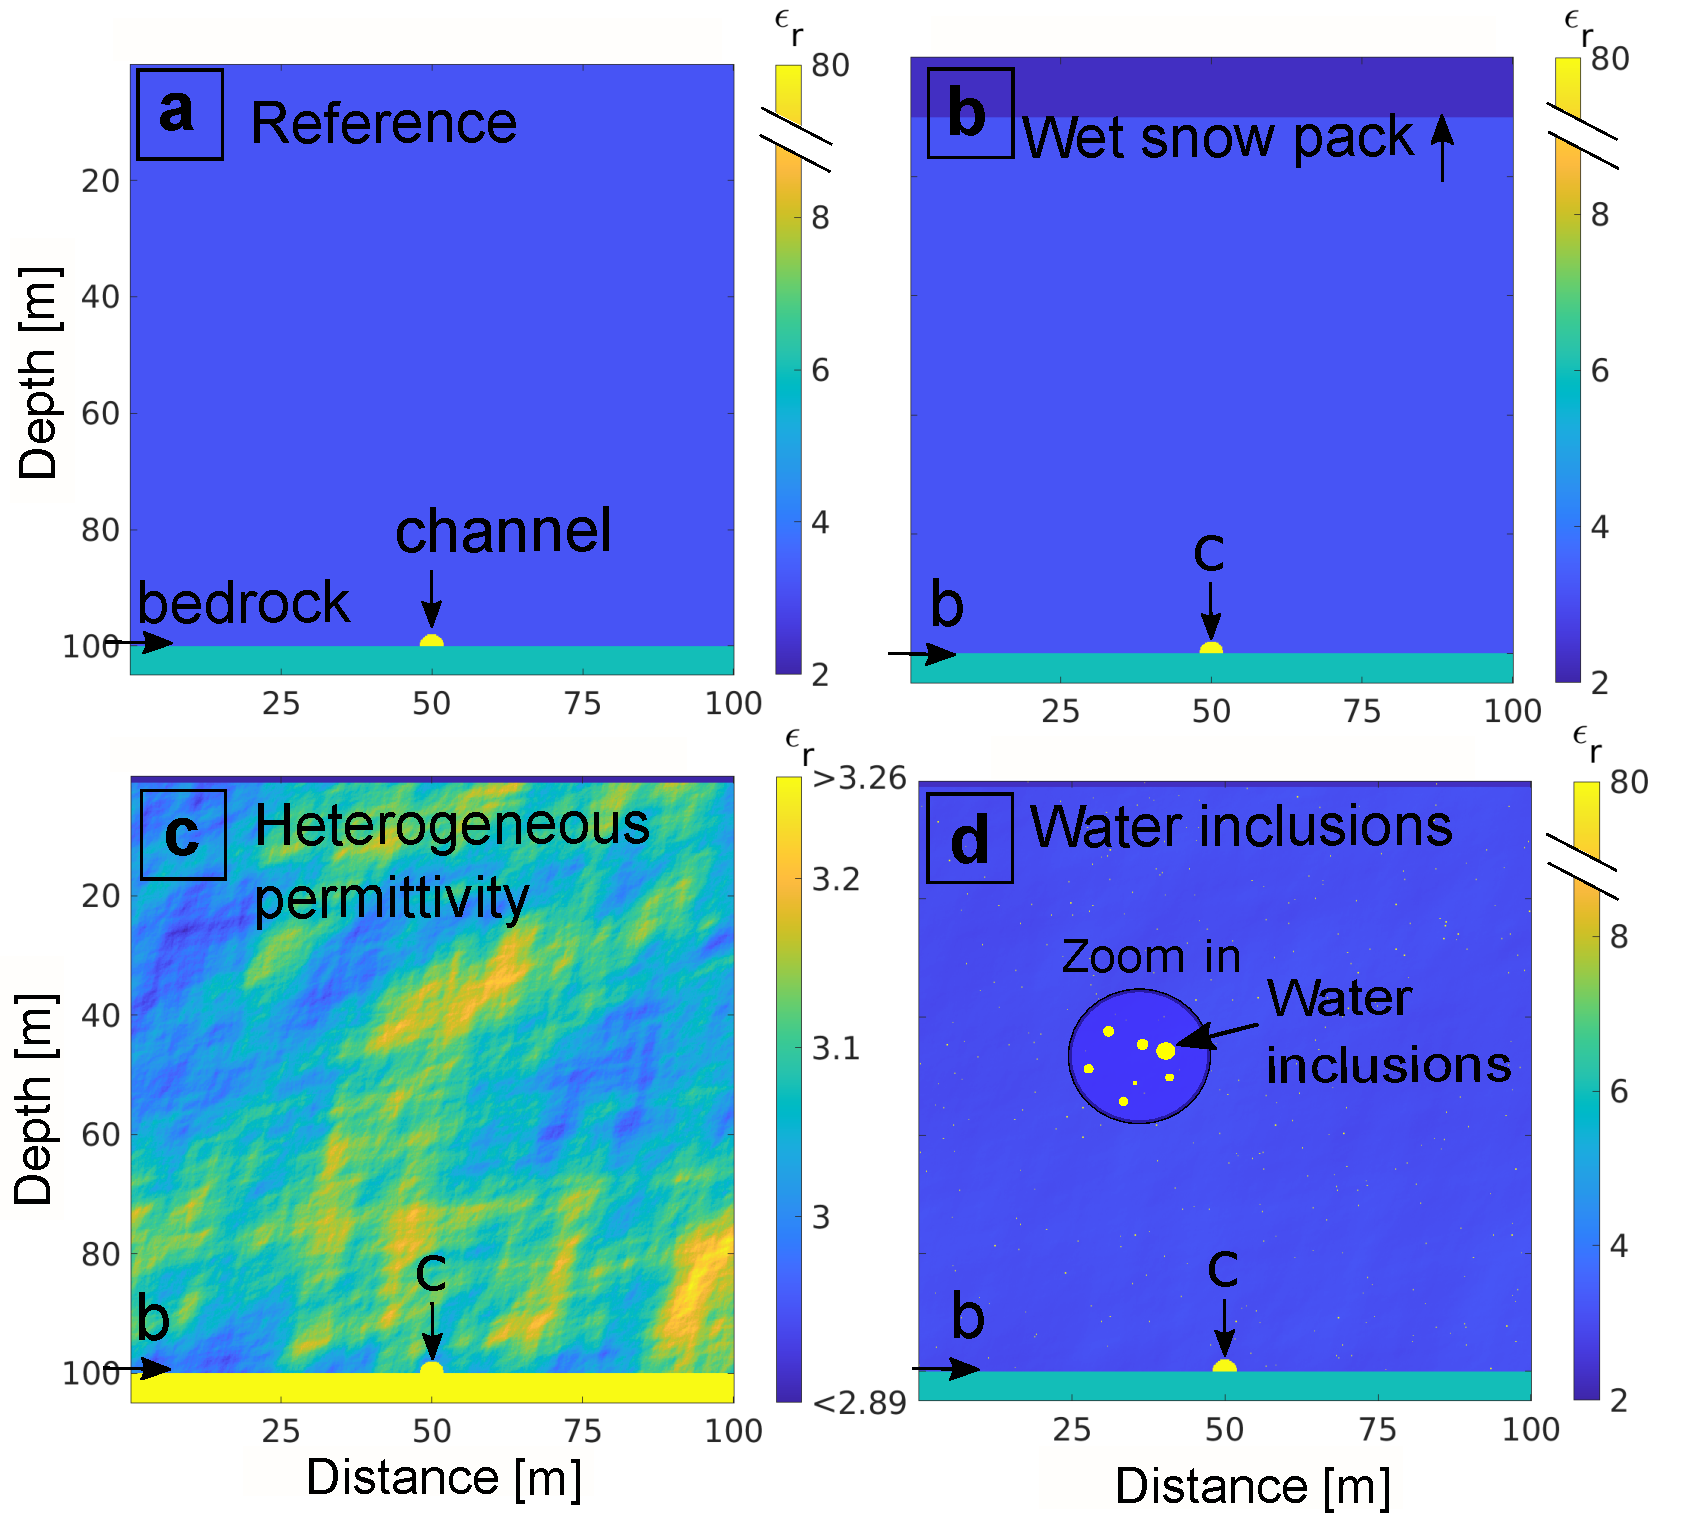
\includegraphics[width=0.6\textwidth]{chapters/chapter_gprmax/Fig01.pdf}
    \caption{2D geometry of the investigated glacier models and relative permittivity ($\epsilon_r$) for (a) the reference model, (b) the additional wet snowpack, here 10\,m thick, (c) the additional stochastic variation of ice permittivity (note the different color scale), and (d) the additional water inclusions (here $LWC$\,=\,0.2\,\% and $r$\,=\,0.1\,m). The position of the bedrock (labeled "b") and the subglacial channel (labeled "c") are indicated by arrows for each model.}
    \label{fig:model_geometry}
\end{figure*}


\subsubsection{Reference model: homogeneous, water-free glacier ice}
\label{sec:ref_model}

The geometry and materials of the reference model are given in Figure~\ref{fig:model_geometry}a. The geometry includes a flat bedrock at 100\,m depth and a subglacial channel with a radius of 2\,m. We include the subglacial channel as a possible target for a GPR campaign. As such, the bedrock and the subglacial channel represent the two targets for which we will check how the imaging quality is affected by the model additions presented below. 


\subsubsection{Model addition 1: wet snowpack at the glacier surface}
\label{sec:snow}

Glacier ice is often overlain by snow or firn, and this layer might contain some liquid water. Such conditions are particularly prominent in spring, when GPR campaigns are often performed \citep[e.g.][]{Bauder&al2018}. We assess the impact of such a layer by adding it to the surface of our reference model (Fig.~\ref{fig:model_geometry}b). The layer thickness is either 1\,m or 10\,m, which we consider being the range of a typical snowpack in Alpine settings. We calculate the layer's permittivity $\epsilon_s$ by using the parametrization suggested by \cite{Tiuri&al1984}: 

\begin{equation}
      \epsilon_s = (0.1\,LWC + 0.8\,LWC\,^2)\epsilon_w + \epsilon_d~,
       \label{eq:epsilon_wet}
\end{equation}

where 0.1 and 0.8 are two empirically determined coefficients, $LWC$ is the liquid water content, $\epsilon_w$\,=\,80 is the relative permittivity of the water (Table~\ref{tab_material_properties}), and $\epsilon_d$ is the relative permittivity of dry snow. The latter is calculated from the density ratio between snow and water, that is $\rho_{snow}/\rho_{w}$ (dimensionless): 

\begin{equation}
  \epsilon_d = 1 + 1.7\times\rho_{snow}/\rho{w} + 0.7\times(\rho_{snow}/\rho_{w})^2~.
  \label{eq:epsilon_dry}
\end{equation}

The wet snow conductivity $\sigma$ ($\mu$S\,m$^{-1}$) is calculated following \cite{Granlund&al2010}:

\begin{equation}
    \sigma \approx  10 + 3\times10^3\,LWC~.
    \label{eq:sigma_wet_snow}
\end{equation}

With the above equations, a typical spring snowpack over glaciers with $\rho_{snow}/\rho_w$\,=\,0.5 and $LWC$\,=\,3\,\% \citep{Griessinger&al2018}, results in $\epsilon_s$\,=\,2.3 and $\sigma$\,=\,10$^{-4}$ S\,m$^{-1}$. These values are in good agreement with field observations (see e.g. Fig.~5 in \cite{Evans1965}). Note that the value for $\epsilon_s$ is close to the permittivity of ice (see Table~\ref{tab_material_properties}), and that we consider a bulk permittivity for the snowpack, i.e. we do not explicitly account for the snowpack's water inclusions. Our argument for doing so is that these water inclusions are expected to be very small when compared to the wavelength of the GPR signal in snow: at 25\,MHz, the latter is in the order of 1\,m, while the diameter of the water inclusions in snow are expected to be <\,1\,mm \citep[e.g.][]{Coleou&al2001}.  

\subsubsection{Model addition 2: heterogeneous ice permittivity}
\label{sec:stoch_mod}

Measurements of the relative permittivity of ice $\epsilon_r$ (dimensionless) range between 2.89 and 3.26, with a mean value of $\sim$3.2 \citep{Reynolds2011, Johari&Charette1975, Robin&al1969, Plewes&Hubbard2001, Bohleber2012, Jezek&al1978}. Variations in  $\epsilon_r$ occur do to the permittivity's dependence on ice density, temperature, and crystal orientation fabrics. The influence of ice density is discussed in \cite{Kovacs&al1995}, who proposed a slightly modified relationship proposed by \cite{Robin&al1969} for capturing such effects. 

Ice density in alpine glaciers is most often considered to be homogeneous, and we thus expect $\epsilon_r$ to vary only little. \citet{Bohleber2012}, for example, reported variations in the order of a few percent (see their Fig.~4). Crystal orientation fabrics can also influence $\epsilon_r$, with variations in the order of 1\,\% \citep{Johari&Charette1975,Fujita&al1993}.

Here, we account for the natural variations in ice permittivity by imposing stochastic variations on $\epsilon_r$ in the range of 2.89 to 3.26 (Fig.~\ref{fig:model_geometry}c). The stochastic distribution is parameterized with a von Karman type correlation function \citep{Goff&Holliger2012} described by a Hurst number 0.5 (that is an exponential distribution) and a correlation length of 10\,m (both in the horizontal and the vertical dimension). The Hurst number (also known as the "fractal dimension") characterizes the amount of heterogeneity in a natural medium \citep{Goff&Holliger2012}, and we will explore the sensitivity of this value in the Results section.


\subsubsection{Model addition 3: scattering water inclusions}
\label{sec:water}

Water inclusions are modelled as randomly distributed, spherical scatterers. We constrain LWC and the size of the scatterers based on literature values. \cite{Barrett&al2008} explain strong scattering in a surging glacier by the presence of water inclusions of multi-decimeter scale. Likewise, \cite{Hodge1976} observed englacial voids in boreholes, reporting that typical vertical extents were of several decimeters (see their Fig.~3).

LWC in temperate ice has been estimated from GPR by analysing the electromagnetic wave velocity \citep{Macheret&al1993,Moore&al1999,Murray&al2000} or from the back-scattered power in individual GPR sections \citep{Bamber1988,Hamran&al1996,Macheret&Glazovsky2000}. Reported LWC values ranges from 0.5\,\% to 1.5\,\% in \cite{Murray&al2000}, from 0.3\,\% to 1.7\,\% in \cite{Raymond&Harrison1975,Vallon&al1976}, and from 0\,\% to 9\,\% in \cite{Pettersson&al2004}. 

More recently, LWC has been estimated from surface nuclear magnetic resonance (SNMR). SNMR is a geophysical technique that allows the direct detection and quantification of liquid water in the subsurface. It takes advantage of the magnetic moment and spin of the hydrogen nuclei of water. Traditionally applied in hydrological applications, the technique has shown promising results in glacier applications too \citep[e.g.][]{Hertrich&al2007,Legchenko&al2011,Garambois&al2016}. In summer 2008, SNMR was for example performed at the tongue of Rhonegletscher, a temperate glacier in Switzerland, yielding an average LWC estimates of 0.8\,\%\,$\pm$\,0.4\,\% for the sampled vertical profile \citep{Hertrich&Walbrecker2008}. 

To test the effect of different configurations of distributed scatterers on the GPR signals, we perform simulations in which we (i) vary the LWC between 0.1\,\% and 1.5\,\%, with increments of 0.1\,\% (i.e. fifteen different values for LWC) and (ii) randomly vary the radius of the water inclusions between 0 and a maximal radius of either r\,=\,0.1\,m, r\,=\,0.5\,m, or r\,=\,1.0\,m. This results in a total of 15\,$\times$\,3\,=\,45 simulations (Fig.~\ref{fig:model_geometry}d provides one example). The position of the scatterers is randomly generated but remains the same for each combination of LWC and $r$. This is to allow for comparisons between simulations. The di-electric properties of the water inclusions are the ones of glacial melt water (see Tab.~\ref{tab_material_properties}). 


\subsection{Numerical modeling and processing of GPR data}

\subsubsection{Modeling algorithm}

For modeling the GPR signal  numerically, we use the open source software gprMax \citep{Warren&al2016}. gprMax implements Yee's algorithm to solve Maxwell’s equations in 2D or 3D using the finite-difference method in the time-domain \citep[FDTD,][]{Kunz&Luebbers1993}. Here, we use the 2D configuration, for which gprMax uses the so-called transverse magnetic mode. This is achieved by setting the length of one of the horizontal dimensions to the spatial discretization, thus reducing that dimension to a single grid point. We use this 2D modeling approach (as opposed to 3D) because GPR field-data are most often migrated in 2D profiles and to reduce computational cost.

The source signal in gprMax is set to a Hertzian dipole with a dominant frequency of 25\,MHz \citep[a typical frequency for investigations on Apline glaciers; e.g.][]{Grab&al2021,Church&al2020} and with a Ricker type source-time function. To mimic field measurements, we place the transmitter and receiver antennas at 0.5\,m above the glacier surface and perpendicular to the investigated profile. The spacing between the transmitter and the receiver is kept constant at 4\,m (corresponding to one wavelength in air at 25\,MHz). The spatial increment of the antennas position along the profile (i.e. the trace spacing) is of 0.5\,m. The length of the GPR profile for each simulations is equal to 95\,m and corresponds to 190 traces. gprMax antennas characteristics are summarized in Table~\ref{table:param_gprmax}. 

In order to run the gprMax simulations, we discretize the glacier models defined in the previous Section in space and time. To avoid numerical dispersion, the space discretization length $\Delta l$ should be $\leq \lambda_{min} / 10$ \citep{Warren&al2016}, where $\lambda_{min}$ is the smallest wavelength of the propagating electromagnetic field. For a given frequency, $\lambda_{min}$ is associated to the material with the smallest electromagnetic propagation velocity $v_{min}$. We calculate $\lambda_{min}$ as follow:

\begin{equation}
   \lambda_{min} = \frac{v_{min}}{f_{max}} = \frac{c}{3\,f\,\sqrt{\epsilon_r}}~,
\end{equation}

where $\epsilon_r$ is the relative permittivity and $f$ the central frequency ($f_{max}$\,=\,3$\times f$ as we consider as null the amplitude beyond three time the central frequency for a Ricker waveform). In our case, $\lambda_{min}$ is found for water, which is the material with the largest relative permittivity (see Tab.~\ref{tab_material_properties}) and thus the smallest velocity ($v_{water}$\,=\,0.33$\times$\,10$^{8}$\,m\,s$^{-1}$). 

For $f$\,=\,25\,MHz and water, $\lambda_{min}$ is 0.44\,m, and we thus chose $\Delta l$\,=\,0.05\,m. This means that the wavelength in the water is sampled by nine cells. The fact that we sample by nine cells instead of ten means that the highest frequency (and thus the shortest wave length) propagates with a velocity on the grid that is 0.93\,\% smaller than the desired velocity \citep{Schneider2010} -- a difference which we consider as being negligible. The time is discretized according to $\Delta l$ and following the Courant-Freidrichs-Lewy stability condition \citep{Warren&al2016}. The receiver recording time is set to 1.5$\times$10$^{-6}$\,s, which corresponds to a penetration depth of the signal in ice of $\sim$\,125\,m (two way travel). A so-called perfectly match layer width of ten cells (i.e., 0.5\,m) is set on the model boundaries to absorb the signal and simulate an unbounded space \citep{Berenger1996}. Time and space model parameters for gprMax are summarized in Table~\ref{table:param_gprmax}.


\begin{table*}
\centering
\caption{Time and space parameters for the gprMax simulations.}
\label{tab_domain}
\begin{tabular}{l c r}
\hline
\textbf{gprMax antenna characteristics}  & \textbf{Value} & \textbf{Remarks} \\
\hline
Frequency & 25\,MHz  \\
Waveform type & Ricker & Amplitude = 0.99\\
Antenna dipole & Hertzian &\\
Antenna separation & 4\,m & \\
Antenna step size & 0.5 m & \\
Antenna height above surface & 0.5\,m & \\
Antenna orientation & & Perpendicular to profile\\
\hline
\textbf{gprMax time/domain parameters}  &  &  \\
\hline
GPR profile length & 95\,m & 190 GPR traces \\
Cell size ($\Delta l$) & 0.05\,m & Frequency dependant\\
Time step & 1.05$\times$\,10$^{-10}$\,s & Frequency dependant \\
Time window & 1.5$\times$10$^{-6}$\,s & Two travel-time \\
Perfectly match layer width & 10 cells & Absorbing layer\\
\hline
\end{tabular}
\label{table:param_gprmax}
\end{table*}

Solving Maxwell’s equations using the FDTD approach for high-resolution data is computationally expensive. To accelerate the simulations, we run gprMax on graphics processing units (GPUs). The FDTD discretization allows for a natural and efficient parallelization of the solver and allows  leveraging the parallel processing capabilities of latest GPUs. We run the simulations using eight Nvidia A100 (SXM4, 40GB) GPUs. gprMax also allows for multi-GPU configurations, where independent trace computations are distributed among GPUs using message passing interface for distributed parallelization in a master-slave configuration. GPU computing permitted to speed up the simulations by a factor of 15 compared to multi-threaded central processing unit configurations. This results in a typical runtime for a single simulation of $\sim$\,5\,min. All data necessary to reproduce our gprMax simulations, including the MATLAB input files generator, are available in the Section Code and Data Availability. 

\subsubsection{GPR data processing}

The gprMax output contains time series of the electromagnetic field strength for all grid cells and for all traces. As for field data, further processing is required to generate GPR sections that can actually be interpreted. For this, we employ our in-house Matlab-based toolbox GPRglaz \citep{Grab&al2018} and follow the processing workflow typically used for field-based investigations \citep[e.g.][]{Church&al2020,Grab&al2021}. 

More specifically the workflow comprises (1) time zero correction based on the arrival of the direct wave, (2) bandpass filtering (10\,MHz to 65\,MHz) to cut undesirable low and high frequencies generated by numerical dispersion, and (3) image focusing and time-to-depth conversion that migrates the data with a constant radar wave velocity \citep[0.167\,m\,ns$^{-1}$ for ice;][]{Glen&Paren1975}. Migration is performed with a Kirchhoff time migration scheme \citep{Margrave&Lamoureux2019}. For access to the generated GPRglaz results, see the Section Code and Data Availability. 


\section{Results}

\subsection{Impact of a wet snowpack and a heterogeneous ice permittivity}

Figures~\ref{fig:model_ref_results}a, \ref{fig:model_ref_results}b and \ref{fig:model_ref_results}c present the GPR-signals from our gprMax simulations for the reference model (i.e homogeneous ice), the additional wet snow pack at glacier surface, and for the additional stochastic distribution of ice permittivity, respectively (see also Fig.~\ref{fig:model_geometry}). Early times carry the signature of the direct wave travelling from the transmitter to the receiver antenna. The bedrock reflection is well visible, and the channel structure manifests itself in form of an X-shaped pattern. This is an artefact from the Kirchhoff migration, which is due to its diffraction-limited characteristic \citep{Ozdemir&al2014}.



\begin{figure*}
    \centering
    \includegraphics[width=0.5\textwidth]{chapters/chapter_gprmax/Fig02.pdf}
    \caption{Results of the gprMax simulations for the (a) reference model, (b) additional wet snowpack, (c) additional stochastic variation of ice permittivity, and (d) additional water inclusions (here $LWC$\,=\,0.1\,\% and $r$\,=\,0.1\,m). The associated geometry and materials are shown in Figure~\ref{fig:model_geometry}. The positions of the bedrock (label "b") and the subglacial channel (label "c") are indicated by arrows for each model. All results are presented for a frequency of 25MHz and after Kirchhoff migration.}
    \label{fig:model_ref_results}
\end{figure*}

The snowpack at the glacier's surface has no visible influence on the signal, even when it has a thickness of 10\,m (see Fig.~\ref{fig:model_ref_results}b). This is in agreement with \cite{Smith&Evans1972}, who stated that GPR signal attenuation of wet firn is relatively small as long as the liquid water is salt-free -- a condition certainly met in Alpine environments. 

A heterogeneous ice permittivity results in small perturbations of the signal (Fig.~\ref{fig:model_ref_results}c). However, the strength of the signals is significantly weaker than the one reflected from the bedrock and the subglacial channel. The statement holds true also when varying the parameters that govern the stochastic distribution of the permittivity (these are the Horst number $\nu$ and the correlation length $\lambda$): Figure~\ref{fig:sensitivity_stoch} shows the results for simulations with $\nu$\,=\,0.1 and $\nu$\,=\,2, as well as $\lambda$\,=\,1\,m and $\lambda$\,=\,20\,m -- a range of values that we assume covering any plausible variations in real-world conditions. Both the resulting field strengths and noise patterns are very similar to Figure~\ref{fig:model_ref_results}c, indicating that the choice of model parameters and, more importantly, of variations in permittivity as such, only have a marginal influence on the retrieved GPR signal. 

\begin{figure*}
    \centering
    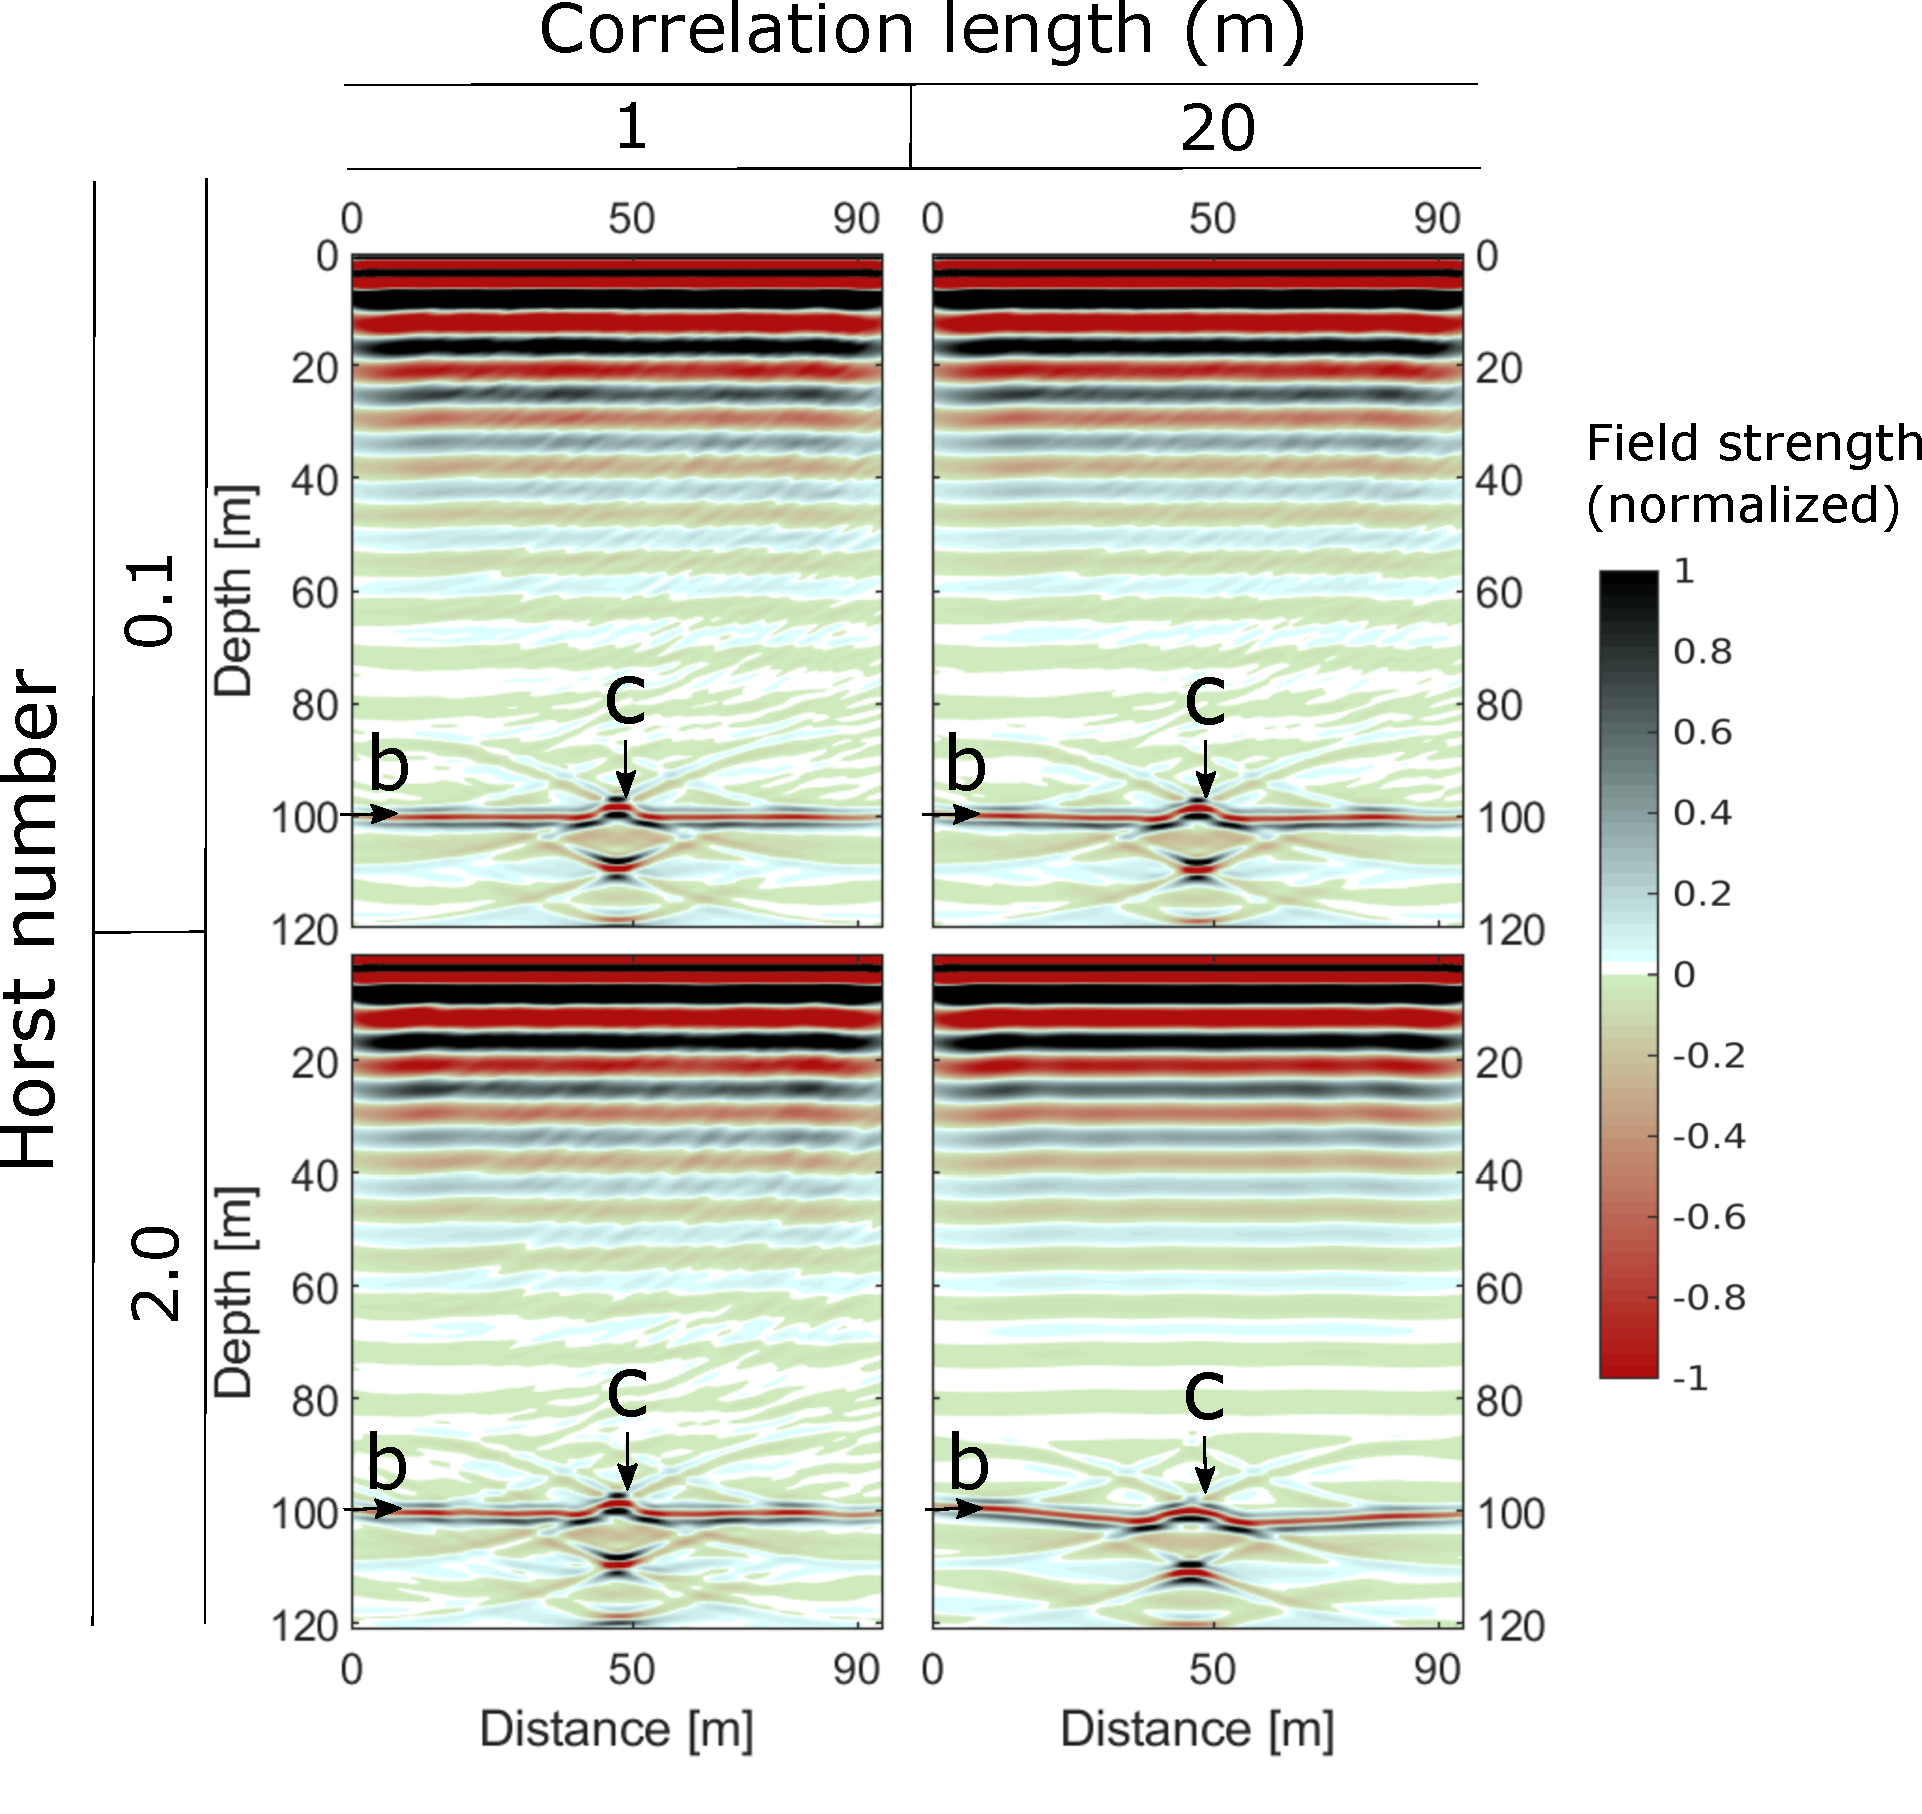
\includegraphics[width=0.5\textwidth]{chapters/chapter_gprmax/Fig03.pdf}
    \caption{Sensitivity test for the Horst number $\nu$ and the correlation length $\lambda$ used for simulating a stochastic distribution of ice permittivity. The range of explored values (i.e. $\nu$\,=\,[0.1,2.0] and $\lambda$\,=\,[1, 10]\,m) are considered to be plausible upper- and lower-bounds. Data are presented after Kirchhoff migration. The bedrock (label "b") and the subglacial channel (label "c") are indicated.}
    \label{fig:sensitivity_stoch}
\end{figure*}

We thus conclude that natural variations in ice permittivity are insufficient to explain the noise that characterizes many GPR data  acquired in the field for temperate glaciers. 


\subsection{Impact of water inclusions}

The impact of water inclusions on the GPR signal is shown in Figure~\ref{fig:model_ref_results}d, and results in a signal that is qualitatively similar to field data (see the Discussion Section for more details). For the chosen parameters (i.e. $LWC$\,=\,0.1\,\%, $r$\,=\,0.1\,m), the bedrock and the subglacial channel remain visible, although much less clearly than for the reference model. 

To further investigate the effects of water inclusions, the simulations are repeated with different LWCs and different sizes of the water inclusions. Figure~\ref{fig:gprmax_results} presents a selection of simulation for three values of each LWC and maximum scatterer radius. In all cases, the GPR signal is strongly attenuated with increasing depth because of the energy lost through scattering. For $LWC$\,=\,0.1\,\% and $r$\,=\,0.1\,m, the bedrock and the subglacial channel are well visible. For higher LWC (e.g. 0.5\,\% and 1\,\%), the bedrock and the subglacial channel are no longer visible, regardless of the radius of the water inclusions. This indicates that bulk LWC values in the range of 0.1\,\%\,-\,0.5\,\%, associated to water inclusions with radii in the order of several decimeters, already constitute a limit beyond which a bedrock at 100\,m depth becomes impossible to detect with a frequency of 25\,MHz. When the scatterer size increases for a constant LWC (i.e. when the number of scatterers decreases), more sections of water-free ice appear between the surface and the bedrock. In these sections, the bedrock is better visible, as see when comparing the results with $r$\,=\,1\,m and $r$\,=\,0.5\,m in Figure~\ref{fig:gprmax_results}.
Also note that the bedrock depth tends to be slightly overestimated with increasing LWC. This is because our Kirchhoff migration ignores the presence of water, i.e. it applies the same velocity of propagation for the electromagnetic field for all materials.

While the results presented so far refer to GPR data collected with 25\,MHz antennas, we note that using different frequencies would qualitatively lead to the same results as long as the size of the scatterers are scaled with the dominant wavelength. For example, using 50\,MHz and scatterers with a radius of 0.5\,m would give the same results as for 25\,MHz and a radius of 1.0\,m. At most, a difference is expected to emerge in the achievable penetration depth and the size of the identifiable features, with higher frequencies having stronger attenuation but better spatial resolution than lower frequencies. One would also expect the appearance of multiple internal reflection when the wavelength of the electromagnetic field in water is significantly smaller than the scatterer radius. For 25\,MHz and 50\,MHz, this is the case for scatterers with $r$\,$>$\,1\,m and $r$\,$>$\,0.5\,m, respectively.


\begin{figure*}
    \centering
    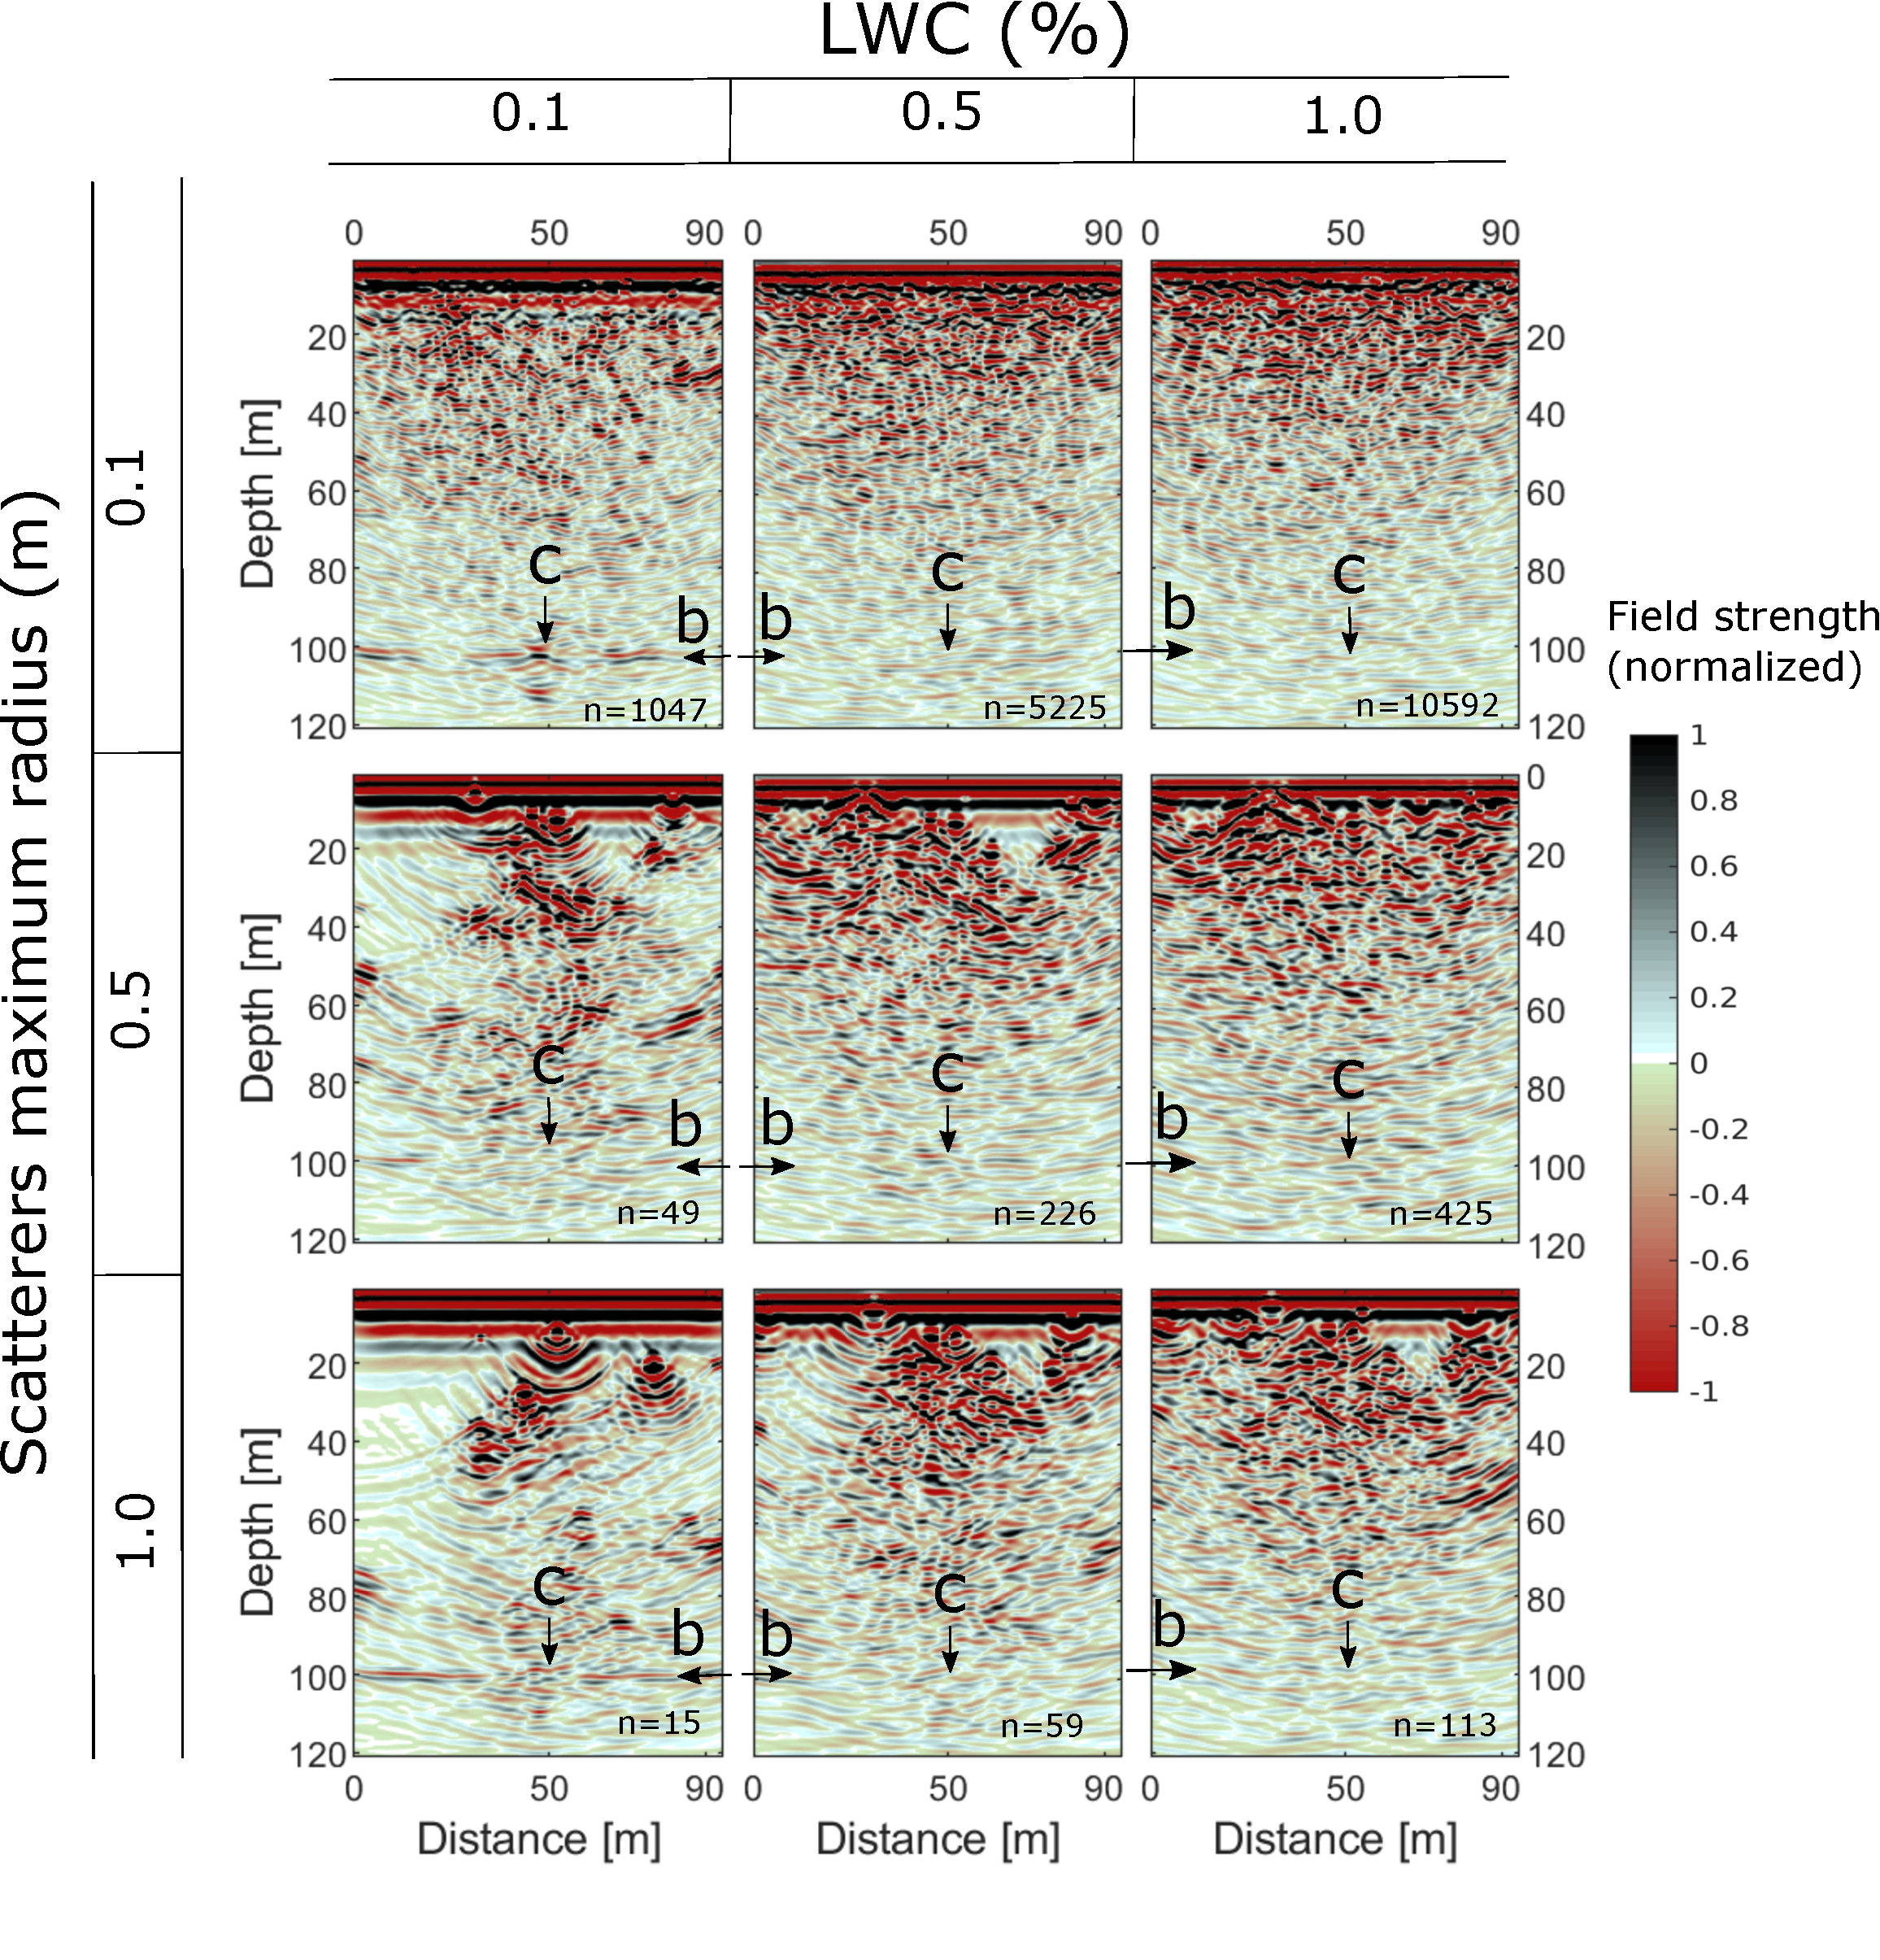
\includegraphics[width=0.5\textwidth]{chapters/chapter_gprmax/Fig04.pdf}
    \caption{Results from gprMax simulations for nine combination of LWC and maximal radius of the water inclusions. The number of individual scatterers $n$ is indicated on the bottom right of each panel. The bedrock (label "b") and the subglacial channel (label "c") are indicated by arrows. Results refer to 25\,MHz and are presented after Kirchhoff migration.}
    \label{fig:gprmax_results}
\end{figure*}


\section{Discussion}

\subsection{Similarities of synthetic and field-data}

Limited bedrock detectability has often been reported \citep[e.g.][]{langhammer&al2017,Grab&al2021,Rutishauser&al2016,Bradford&al2009}. Figure~\ref{fig:field_vs_gprmax}a and \ref{fig:field_vs_gprmax}b present two GPR sections acquired in August 2021 on Glacier du Trient (Switzerland), and in July 2021 on Triftglestcher (Switzerland's Mattertal), respectively. Both glaciers are temperate, and the surveys were carried out with 25\,MHz antennas. The GPR data were processed with GPRglaz using the same steps as described for the gprMax simulations.

For both the mentioned GPR sections, signal scattering is particularly pronounced at depths between 20\,m and 60\,m. The strong bedrock is well visible at depths between 110\,m and 130\,m for Triftgletscher and between 70\,m and 100\,m for Glacier du Trient, but the signal is not continuous across the profiles. Figure~\ref{fig:field_vs_gprmax}c presents one of the synthetic GPR sections, generated with gprMax with $LWC$\,=\,0.1\,\% and $r$\,=\,0.1\,m (same configuration as in Figure~\ref{fig:gprmax_results} and same geometry as in Figure~\ref{fig:model_geometry}d). The spatial pattern of the scatterers and the strength of the reflected energy are very similar to the real-world data shown in Figure~\ref{fig:field_vs_gprmax}a and \ref{fig:field_vs_gprmax}b. This similarity is only achieved when water inclusions are included in our numerical simulations, meaning that the variations in ice permittivity and the presence of a snowpack are not sufficient to reproduce the signal characteristics observed in actual field data. 


\begin{figure*}
    \centering
    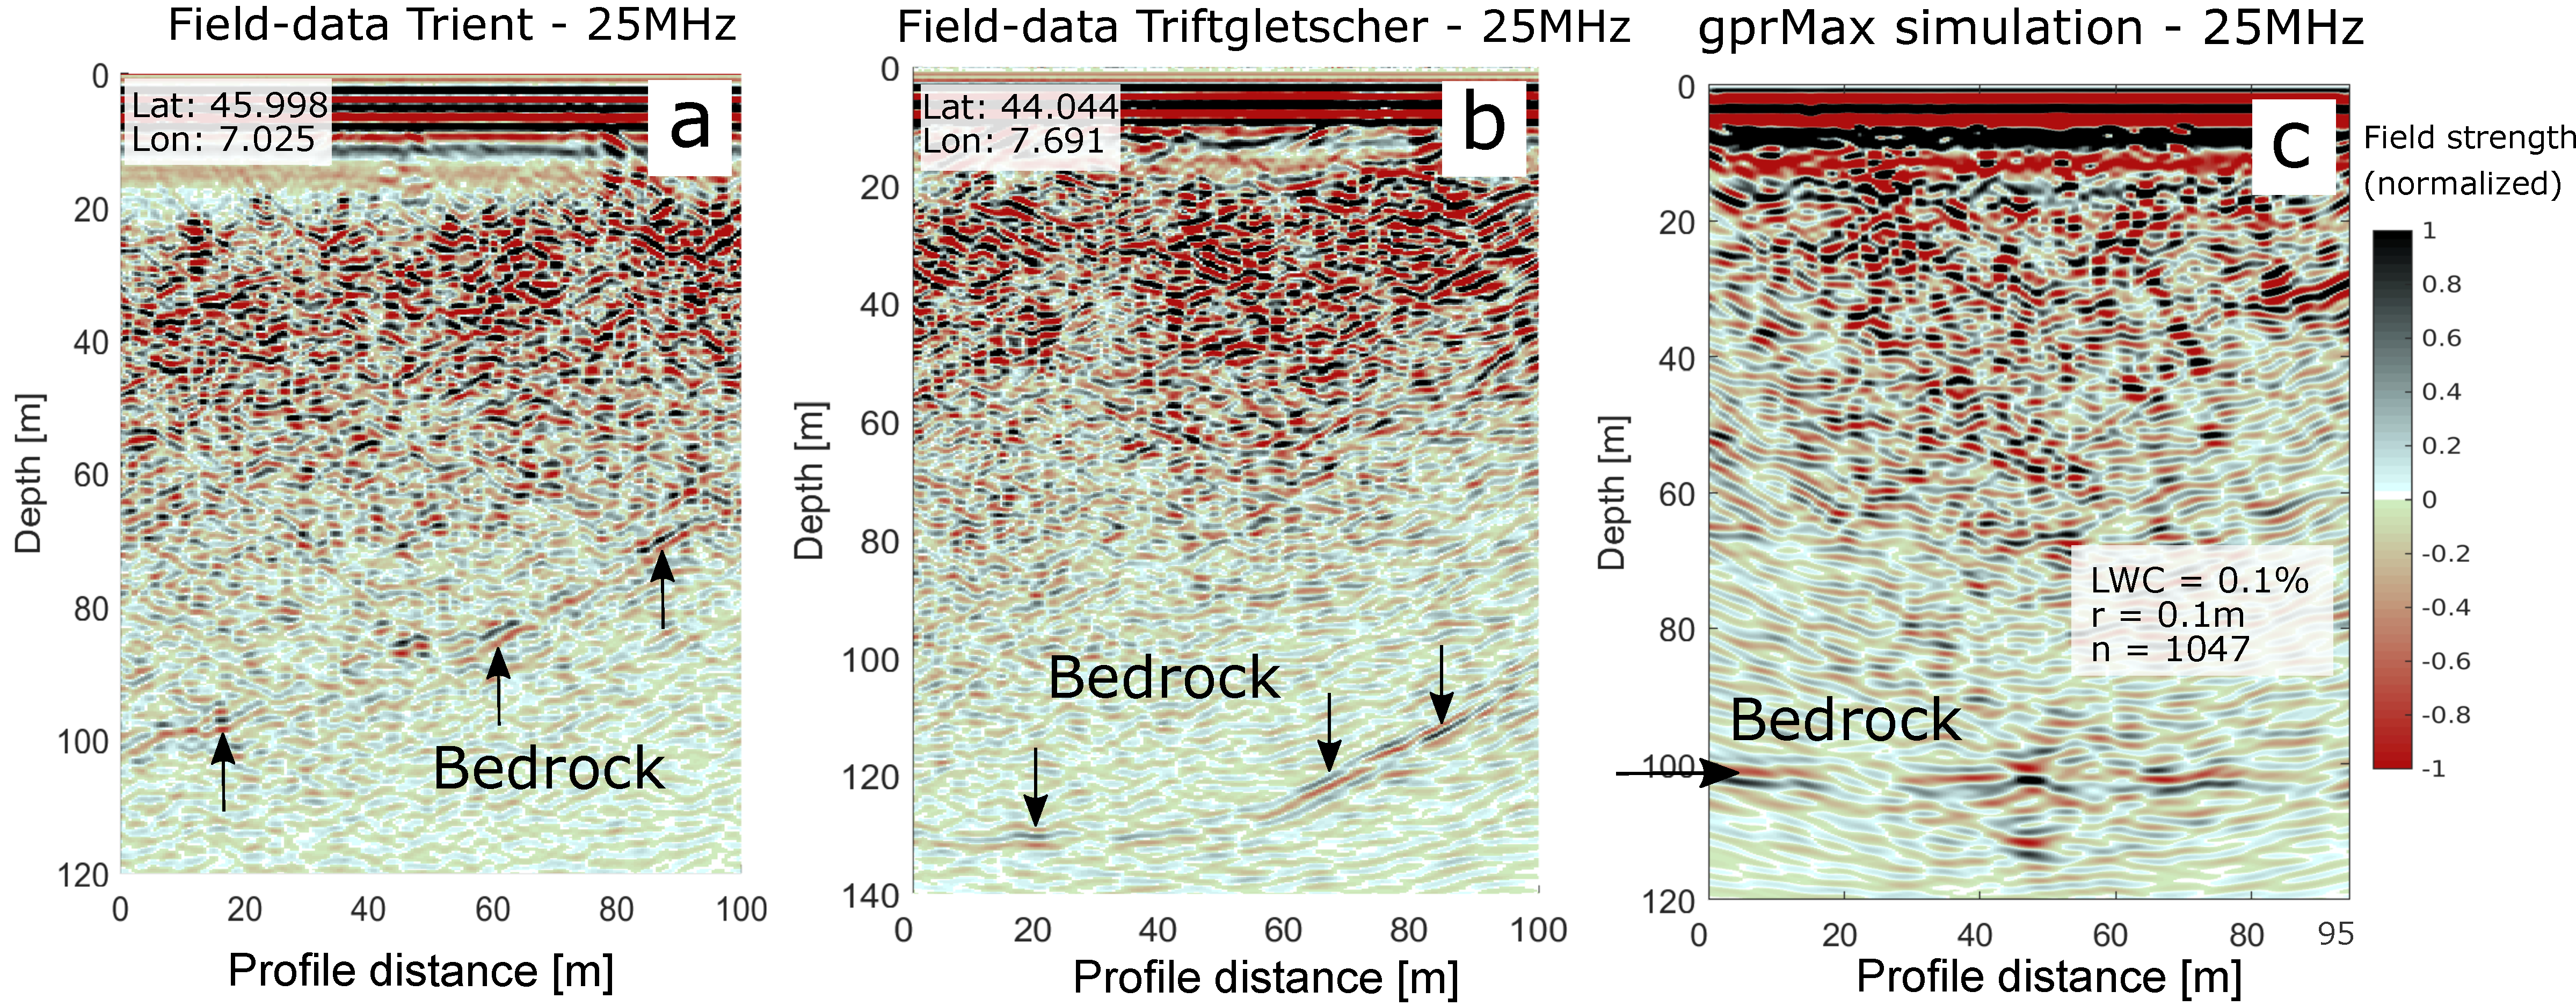
\includegraphics[width=0.5\textwidth]{chapters/chapter_gprmax/Fig05.pdf}
    \caption{Comparison between real-world GPR data and data simulated through numerical modeling. Field data are shown for (a) Glacier du Trient and (b) Triftgletscher (Mattertal), two temperate glaciers in Switzerland. The data simulated with gprMax (c) are obtained with $LWC$\,=\,0.1\,\% and $r$\,=\,0.1\,m, resulting in $n$\,=\,1047 individual scatterers. The bedrock is indicated by black arrows. All three example refer to 25\,MHz antennas and are presented after Kirchhoff migration.}
    \label{fig:field_vs_gprmax}
\end{figure*}


\begin{figure*}
    \centering
    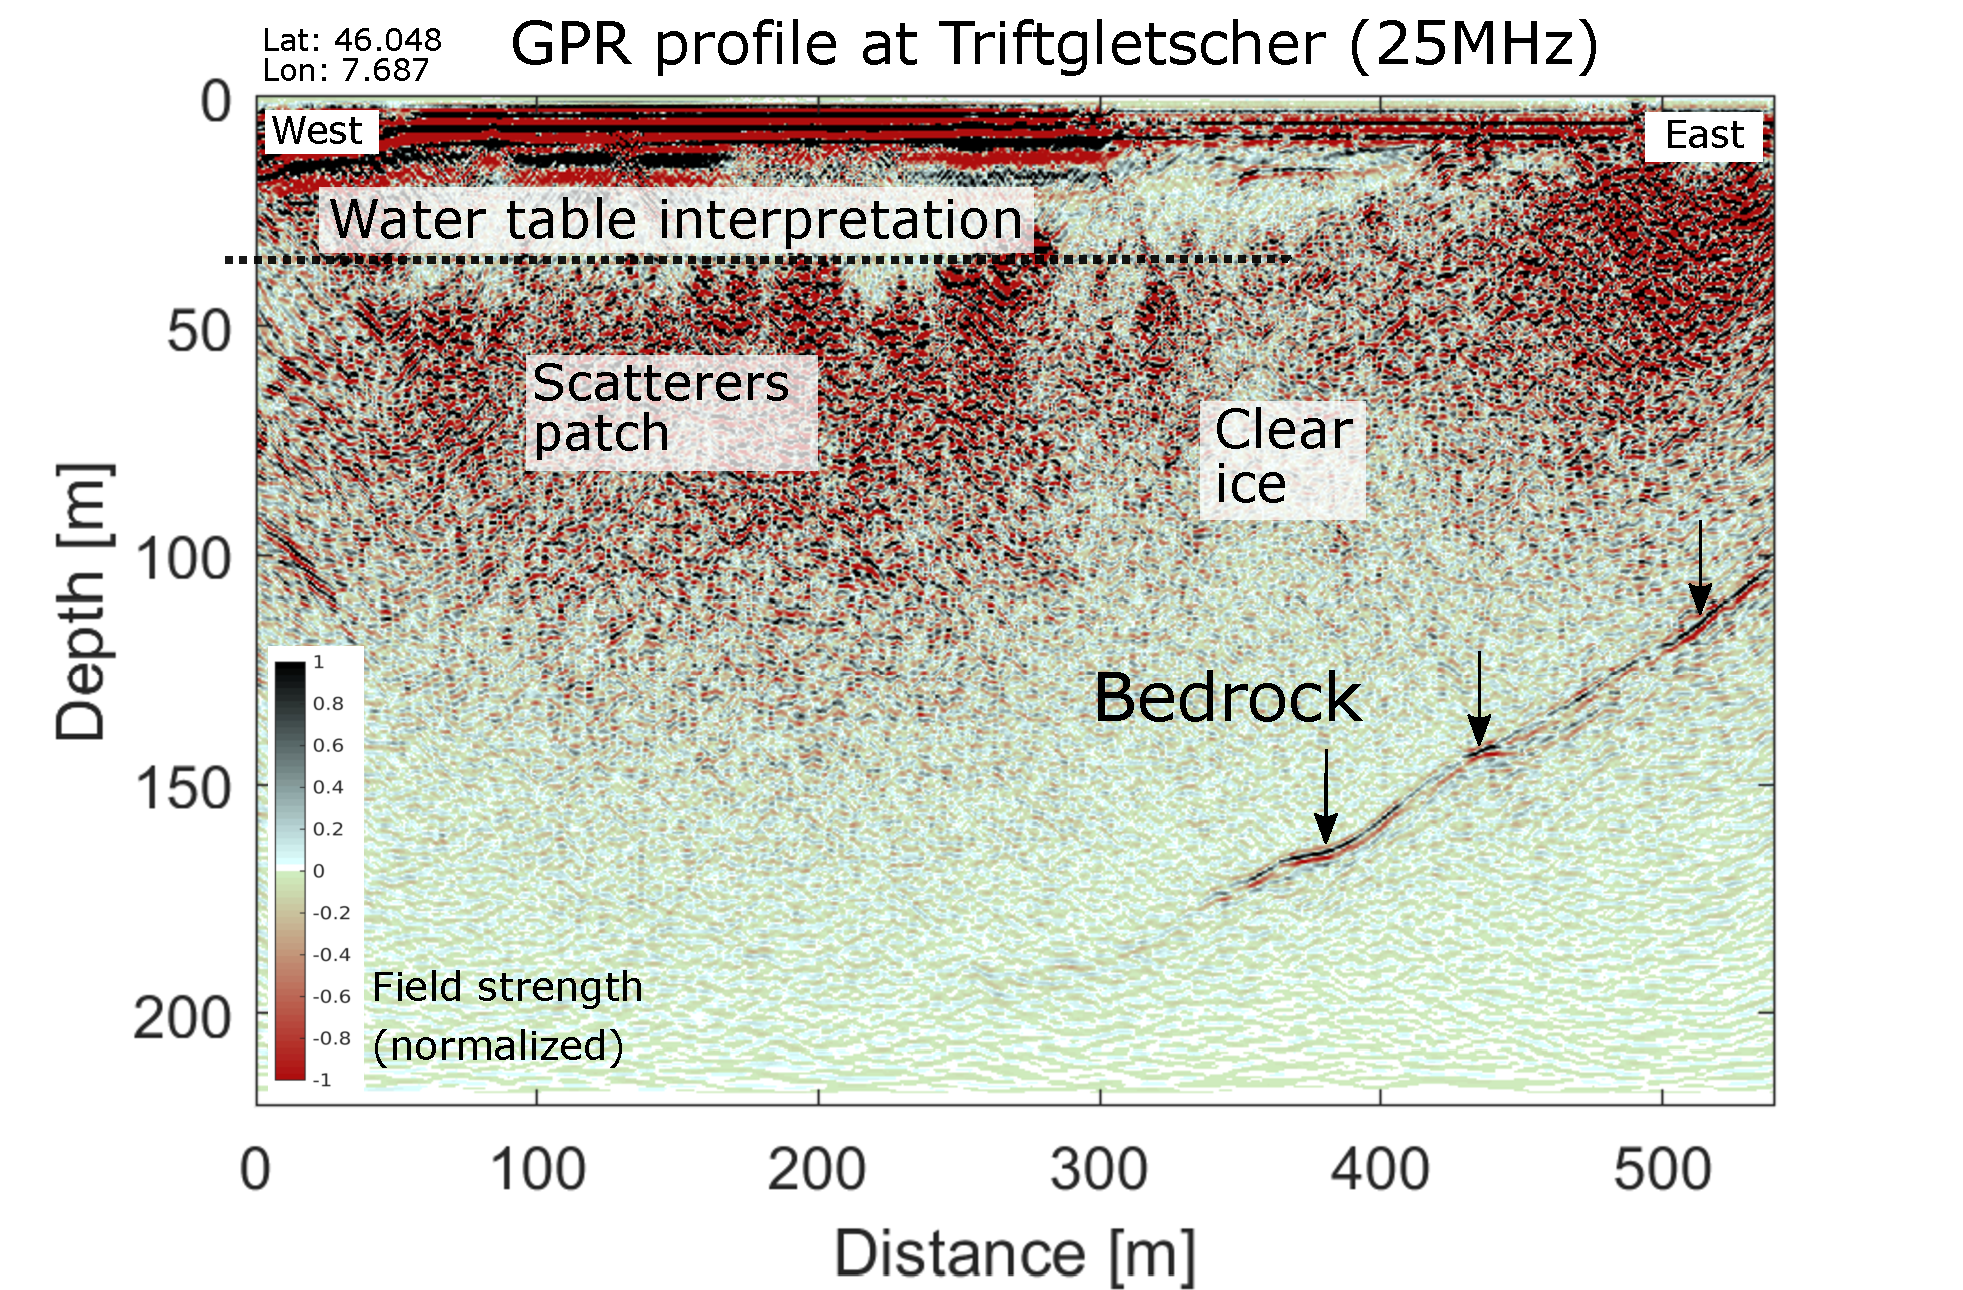
\includegraphics[width=0.5\textwidth]{chapters/chapter_gprmax/Fig06.pdf}
    \caption{GPR field data after Kirchhoff migration on Triftglestcher (July 2021). The depth of the interpreted water table is marked by the horizontal dotted line above the scatterers.}
    \label{fig:trift}
\end{figure*}

\subsection{Scatterer distribution within the glacier body}

A simplification of our analyses is that the scatterers are distributed homogeneously in the entire glacier body. In reality, this might be different. It is known, for example, that the water level within a glacier can fluctuate in space and time as a response to pressure changes in the subglacial drainage system \citep[e.g][]{Iken&al1996,Werder&al2010,Rada&Shoof2018,Graff&Walter2021}. In such cases, one would expect the scattering water inclusions to be preferentially located below an englacial water table. 

Such a distribution is suggested, for example, by a second GPR section collected at Triftgletscher (Fig.~\ref{fig:trift}). At horizontal distances between 0 and 450\,m, the uppermost 30\,m of the ice show an almost scatter-free, transparent zone (note that the some parts of this zone are partially obscured by remnants of the direct wave) while below that level, pronounced scattering is visible. Interestingly, the amount of scattering varies horizontally: between about 300 and 450\,m horizontal distance, for example, the scattering decreased significantly, and as a consequence, the bedrock is clearly recognizable up to a depth of $\sim$\,170\,m. This is in contrast to the GPR section between 0 and 300\,m horizontal distance, where strong scattering obscures the bedrock.

We speculate that high amounts of scattering occur for ice sections with high LWC, e.g. in areas where englacial fracturing is more pronounced due to extensional strain \citep{Bradford&al2009} and where the resulting englacial voids are filled with water. To support this conjecture, we perform another set of numerical simulations in which we subdivide the ice column in two layers: an upper layer with no scatterers (i.e. $LWC$\,=\,0\,\%) and a lower layer, containing all the scatterers. Results for $LWC$\,=\,0.2\,\% and $r$\,=\,0.1\,m are presented in Figure~\ref{fig:sensitivity_bilayer}. A LWC of 0.2\,\% is chosen because the bedrock reflections already start to be obscured in this case  (see Fig.~\ref{fig:gprmax_results}) and because our interest is in exploring the limits of detectability of both the bedrock and the subglacial channel.

For this two-layer configuration, the reflections stemming from both the bedrock and the subglacial channel are qualitatively similar to the one-layer case. We suggest that the reflected signal attenuation is more sensitive to LWC and scatterer-size than to the distribution of the layering. This supports the interpretation that the noisy patches often observed in field data correspond to regions with dense scatterers, the latter being in turn an expression for locally high LWC values. 

The change between regions of weak and strong scattering has been often interpreted as a transition between cold and temperate ice \citep[e.g.][]{Moore&al1999,Blatter&Hutter1991,Bjornsson&el1996}. This is consistent with the interpretation provided above, as cold ice is expected to have only very low LWC and thus only very few and small water inclusions that could produce scattering. However, we note that scatter-free ice section found for Triftgletscher (Fig.~\ref{fig:trift}) is temperate, not cold (this information is derived from in-situ temperature measurement (not shown) that we conducted in the middle of the shown profile at 15\,m depth during August to September 2021). We therefore suggest that temperate ice with very low LWC can have a similar GPR-signature than cold ice. In turn, this indicates that the precise characterization of the thermal regime of a glacier from GPR data alone could be more challenging than assumed so far.  

\subsection{Interpretation of the LWC variations with depth}
\label{sec:LWC_GPR}

The observations made in Figure~\ref{fig:trift} (low scattering near the surface and much more pronounced scattering at depth) have been made on a number of other temperate glaciers too \citep[see, e.g.,][and references therein]{Rutishauser&al2016}. \cite{Rutishauser&al2016} denoted these features as “internal reflection bands” (see their Fig.~13).

Our hypothesis is that such differences in scattering are caused by small-scale water inclusions and by LWC variations with depth. This hypothesis is not only supported by the striking similarity between our modeling results and field data (see previous Section) but also by independent field observations. Indeed, the already mentioned SNMR measurements performed on Rhonegletscher in 2008 \citep{Hertrich&Walbrecker2008}, indicate such LWC variations, with $LWC$\,$\sim$\,0.3\,\% at 30\,m below the surface and $LWC$\,>\,1\,\% below $\sim$\,60\,m. 

A qualitatively similar LWC-profile was found by \cite{Bradford&al2009} for a temperate Alaskan glacier. By analyzing GPR velocity profiles, they distinguished two distinct ice layers: a $\sim$\,20\,--\,30\,m thick layer with LWC between $\sim$\,0\,\% and 0.5\,\% near the surface, underlain by a layer with LWC of $\sim$\,1\,\% to 2.5\,\% (see their Fig.~6).

Also \cite{Murray&al2000} found a layered LWC structure for a temperate Icelandic glacier. Their Figure~8 shows LWC\,$\sim$\,0.2\,\% at the surface and a sharp increase to $\sim$\,3.5\,\% at 28\,m depth. Conversely to our Rhone data, however, \cite{Murray&al2000} found that the LWC decreases again with increasing depth, until reaching $\sim$\,0.1\,\% at the bedrock.

While the field methodologies mentioned above do not allow identifying  sharp transitions in LWC, we suggest that these marked LWC changes can be interpreted as indicative for the presence of a "water table", i.e. a feature similar to what is found for aquifers. In this scenario, ice fractures and other voids that are present below a certain depth would be water filled, while similar features above that level would be filled with air. This interpretation is broadly consistent with observations performed during drilling campaigns on temperate glaciers: boreholes drilled in temperate glaciers generally fill with water up to a certain level, that level being in hydrostatic equilibrium with the subglacial drainage system \citep[e.g][]{Iken&al1996,pohle&&2022}. With this interpretation, the finding by \cite{Murray&al2000} (i.e. the fact that LWC decreases again close to the bedrock) could be explained by the fact that the ice overburden pressure increases with depth, thus tending to re-close any voids that might emerge.

\begin{figure*}
    \centering
    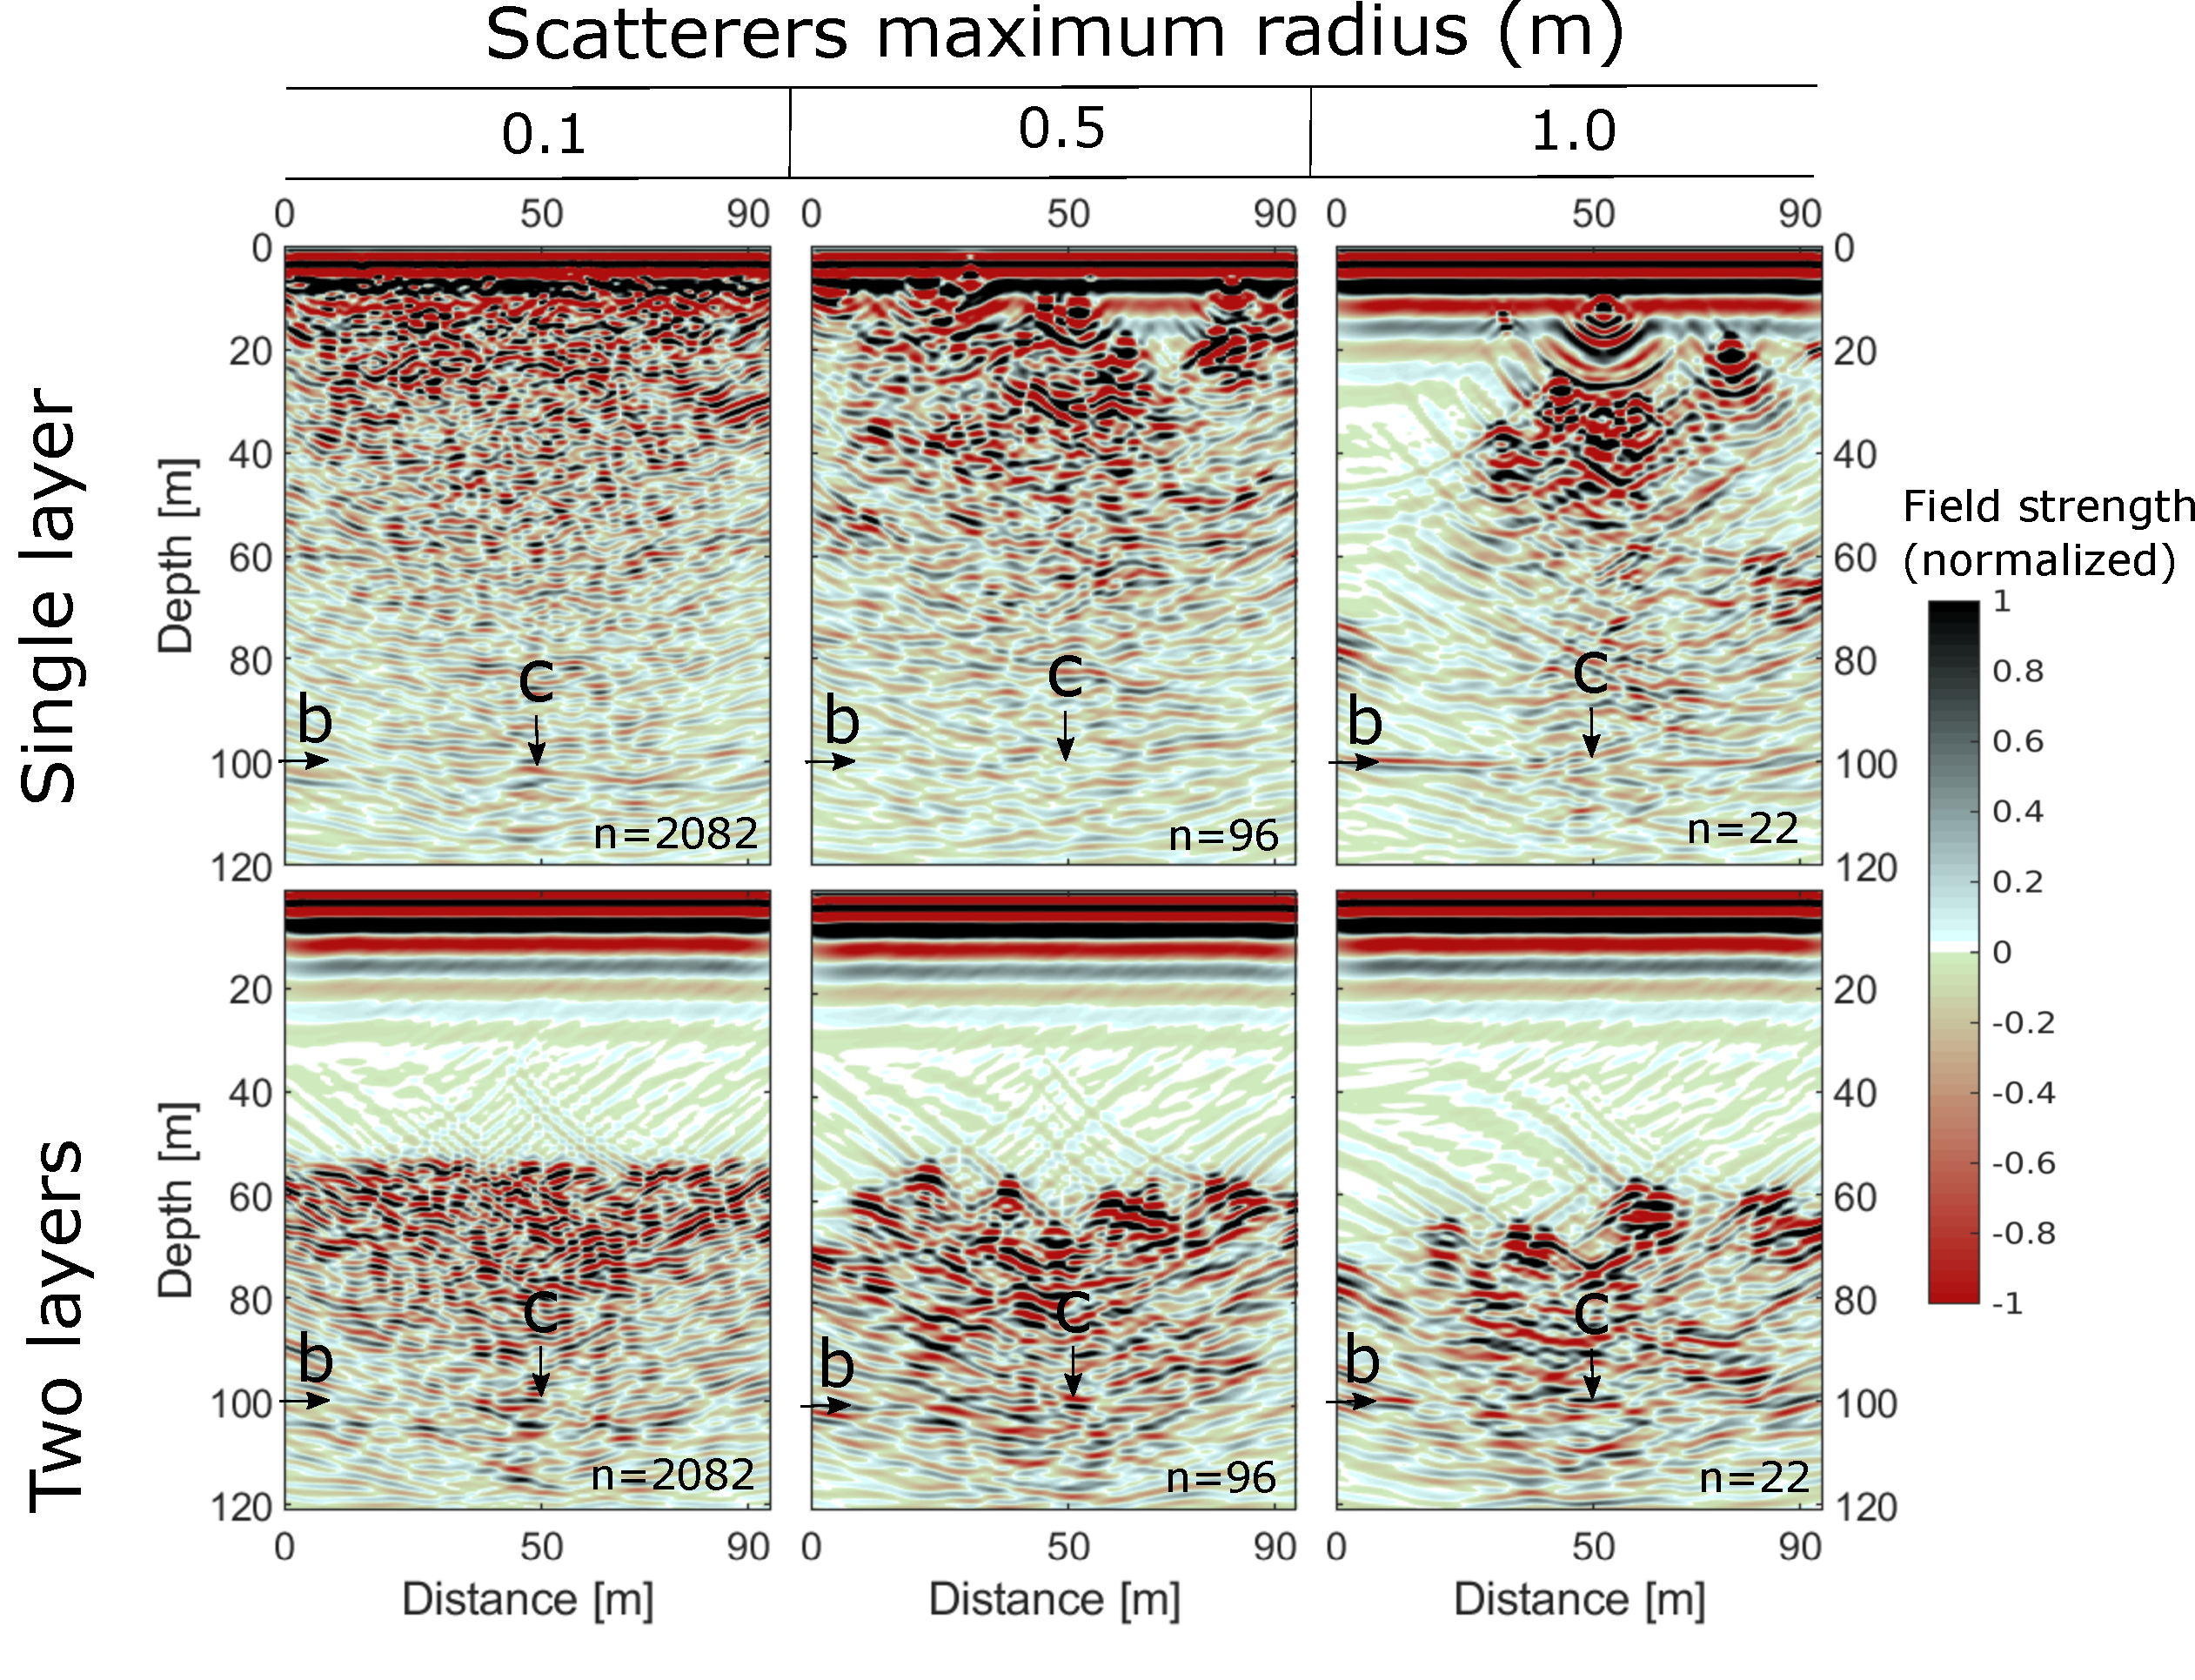
\includegraphics[width=0.5\textwidth]{chapters/chapter_gprmax/Fig07.pdf}
    \caption{gprMax results for scatterers distributed (a) along the entire ice column (labeled "single layer") and (b) only in the lower half of the ice column (labeled "two layers"). $LWC$\,=\,0.2\,\% for all simulations. The number of scatterers $n$ is indicated at the bottom right of each panel. The bedrock and the subglacial channel are indicated by the arrows with labels "b" and "c", respectively.}
    \label{fig:sensitivity_bilayer}
\end{figure*}


\subsection{Plausibility of the size of the water inclusions}

In our simulations, we chose to limit the maximal radius of the water inclusions to $r$\,=\,1\,m. For one, this choice allowed for obtaining a GPR signal that is qualitatively similar to real-world GPR data. For another, these dimensions are broadly compatible with indications found in the literature.

\cite{Holmlund1988}, for example, visually observed former water-filled pockets visible at the surface of a polythermal glacier in Sweden after the surface melted out. Figure~8 and 9 of that publication suggest that these water-filled pockets can be several meters large.

\cite{Bradford&al2009}, as another example, performed GPR velocity analysis in a temperate Alaskan glacier to infer its LWC. They concluded that most of the englacial water is likely to be contained within voids having dimensions in the order of a few centimeters up to several meters, rather than at the ice grain boundaries. 

Further literature examples are difficult to find, and we thus affirm that the question about the size and number of water-filled voids in temperate glaciers merits further attention. 



\subsection{Influence of scatterer distribution and ice permittivity}

So far, the spatial distribution of the scatterers was kept unaltered. This allowed direct comparison of the different simulations. Here, we address the sensitivity of our results to the scatterer distribution by running four gprMax simulations with $LWC$\,=\,0.2\,\% and $r$\,=\,0.1\,m but by changing the scatterer locations. All models have a comparable number of scatterers, although the number is not exactly the same since the radii of the scatterers are randomly varied too. We call the four generated distributions "s1" to "s4" (Fig.~\ref{fig:sensitivity_rng}). 

Figure~\ref{fig:sensitivity_rng}a suggests that for a large number of scatterers, the spatial distribution has little impact on the signal. This is because the scattering is strong everywhere. When the LWC is small and/or scatterers are large (i.e. when scatterers are sparse), we observe a higher sensitivity of the distribution on the signal noise (Fig.~\ref{fig:sensitivity_rng}b). Strong and uniform noise in the GPR signal is thus most likely due to a large number of relatively small scatterers. 

\begin{figure*}
    \centering
    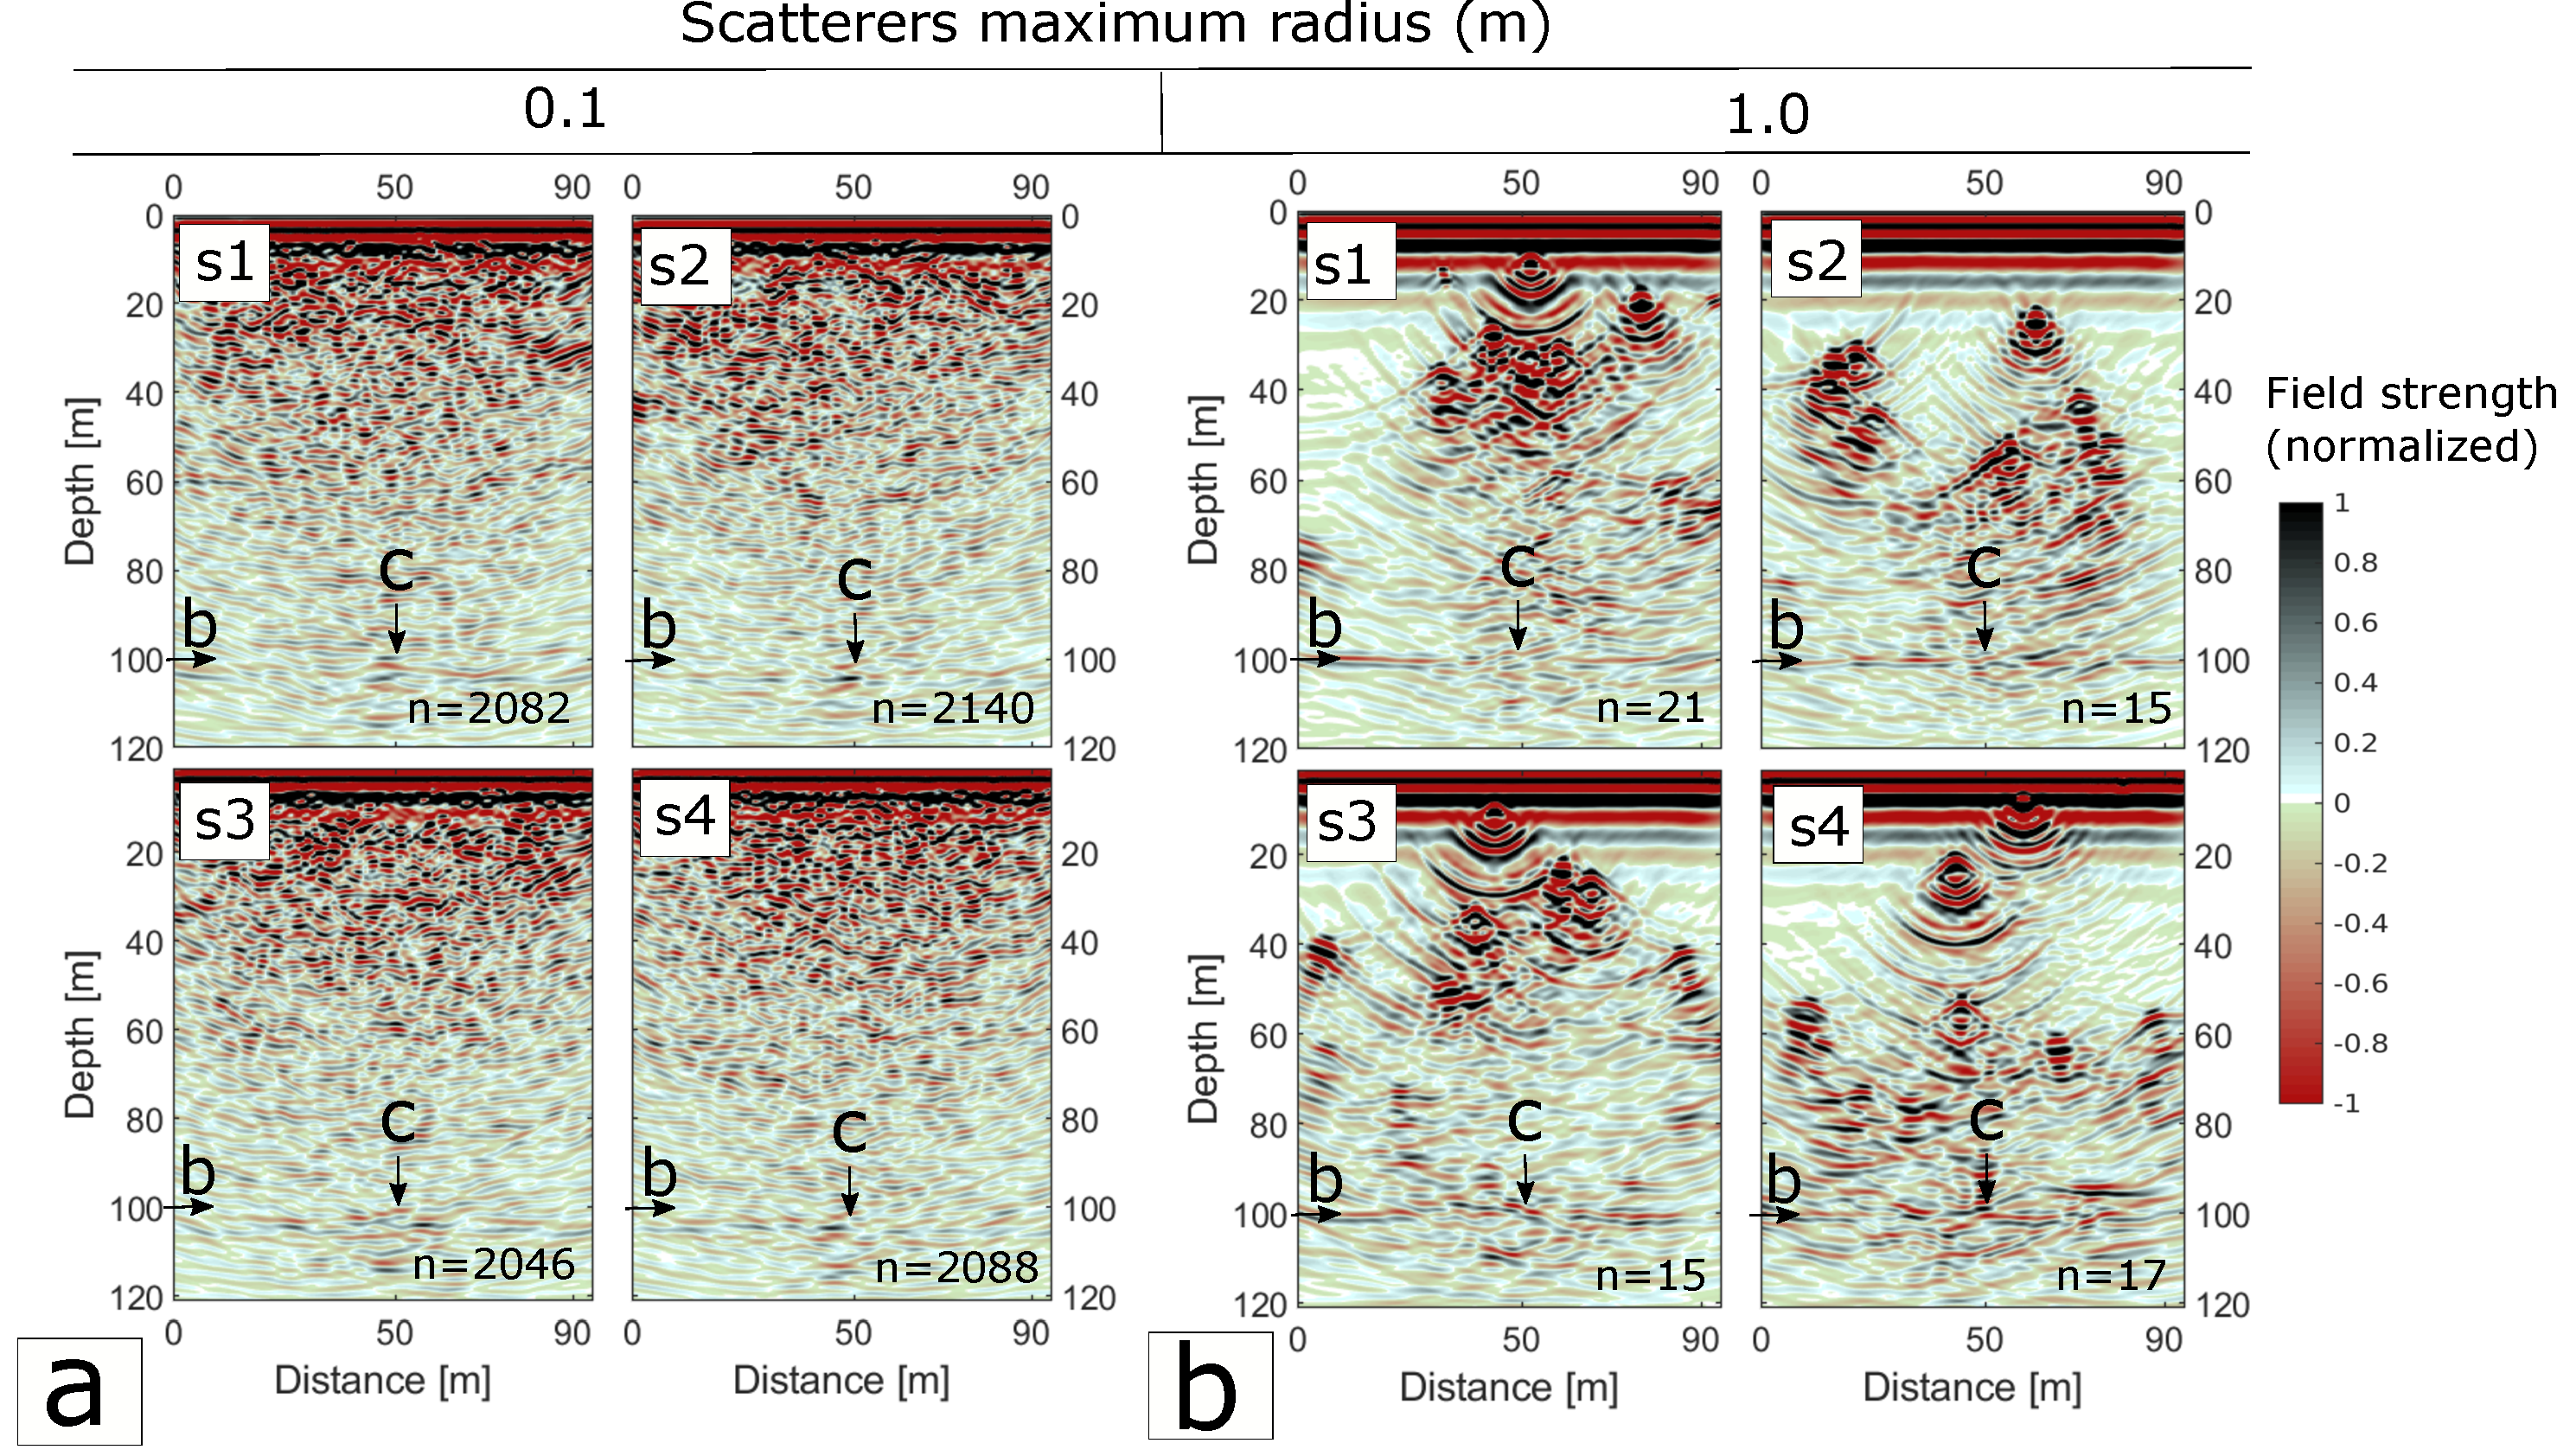
\includegraphics[width=0.5\textwidth]{chapters/chapter_gprmax/Fig08.pdf}
    \caption{Sensitivity test for four different distribution of scatterers (s1 to s4). All panels have $LWC$\,=\,0.2\,\% while the radius of the scatterers is either (a) $r$\,=\,0.1\,m  or (b) $r$\,=\,1.0\,m. The number of scatterers $n$ is approximately the same for all cases (indicated at the bottom right of each panel) while the location of the scatterers is randomly varied. The bedrock and the subglacial channel are indicated by the arrows with labels "b" and "c", respectively.}
    \label{fig:sensitivity_rng}
\end{figure*}


\subsection{Limitations of the method and neglected factors}

Strictly speaking, the detection and imaging of isolated englacial features would require a 3D approach including a dense grid of GPR profiles. This is because side reflections from off-plane scatterers also affect the GPR signal -- a situation that is neglected when applying a 2D migration \citep[e.g.][]{Barrett&al2008}. Although we ignored such effects in our study, the fact that our results look very similar to field data (Fig.~\ref{fig:field_vs_gprmax}) indicates that the first-order effect of water inclusions was sufficiently captured. Our main conclusion is, thus, that small-scale water inclusions are the main reason for the typical scattering observed in GPR data for temperate glaciers.

Related to the above, it is conceivable that other, non-considered englacial features may contribute to the scattering too. Such features could include internal ice structures such as deep crevasses, or moraine material (e.g. rocks) buried within the ice. While such rock inclusions could be of similar size than the water inclusions we considered (diameters ranging from a few millimeters to a few meters) we note that the permittivity of rock ($\epsilon \sim$\,3\,--\,6) is much closer to the one of ice ($\epsilon \sim$\,3.2) than it is to the one of water ($\epsilon \sim$\,80; see Tab.~\ref{tab_material_properties}). This means that the back-scattered energy from a signal originating from rocks is expected to be much weaker than the one from water inclusions, and a similar argument applies to potentially air-filled crevasses (for air, $\epsilon \sim$\,1). Moreover, the typical pattern of moraines and crevasses at the surface of a glacier, i.e. the fact that such features follow a rather clear spatial distribution, suggests that moraine materials and englacial crevasses are likely less ubiquitous than water inclusions. Combined, these two arguments let us argue that although englacial crevasses and rock inclusions might influence the GPR signal, they are very unlikely to be the main source of scattering.


\section{Conclusions}

In this study, we used numerical modeling of GPR signals to characterize the influence that a wet snowpack, a heterogeneous ice permittivity, and distributed water inclusions have on GPR data acquired on temperate glaciers. We showed that the presence of wet snow and heterogeneous ice permittivity are insufficient to explain the strong signal scattering often observed in the field, and instead suggest that englacial water inclusions are the main cause for such scattering.

Our numerical simulations also indicate that a bulk LWC of 0.2\,\%, associated to decimeter-scale water inclusions, is already sufficient to mask bedrock reflections through signal attenuation. The value is in the range of field-based LWC observations, thus explaining why real-world GPR data on temperate ice often fail to detect the bedrock. Our numerical experiments also showed that the GPR signal is sensitive to heterogeneous distributions of water inclusions. In particular, glacier sections with locally low LWC can be far less affected by scattering than sections with high LWC. This gives rise to individual sections that are "transparent" to the GPR signal, i.e. sections with strong signal reflections from the targeted objects.

In terms of practical implications, our results confirm that GPR surveys aiming at estimating subglacial characteristics of temperate glaciers are best conducted in winter, when englacial water contents are generally low and the related scattering is suppressed. In such water-free conditions, temperate ice can have a GPR signature that is similar to the one of cold ice. This implies that distinguishing between cold and temperate ice through GPR surveys -- as sometimes done in the literature -- bares some pitfalls: while the presence of substantial scattering in the GPR signal can be interpreted as indicative for the presence of water and thus temperate ice, the absence of such scattering is indeed indicative for low water contents but these might occur for both temperate and cold ice. Overall, our results contribute to a better understanding and interpretability of GPR signals over temperate ice.


\section{Code and data availability}

The GPR measurements acquired at Triftgletscher and Glacier du Trient are available through ETH Zurich's Research Collection, \url{https://doi.org/10.3929/ethz-b-000590672}. The ice temperature measurements acquired at Triftgletscher are available through ETH Zurich's Research Collection, \url{https://doi.org/10.3929/ethz-b-000609144}. The results of the gprMax simulations and the MATLAB scripts to generate the gprMax input are available through ETH Zurich's Research Collection, \url{https://doi.org/10.3929/ethz-b-000609177}. gprMax is an open access software available at \url{https://www.gprmax.com/}.


\section{Acknowledgements} 

This project was financially supported by the Swiss National Science Foundation (grant nr.\,200021\_212061).
The authors thank the following persons for their support during the fieldwork at Triftgletscher and Glacier du Trient in 2021: Raphael Moser, Guillem Carcanade, Mathieu Cretet, Clement Valla, Lea Geibel, Manuela Köpfli, Lena Strauman, Josquin Pfaff and Inés Dussaillant.
